\begin{figure}[!htb]
	\begin{center}
  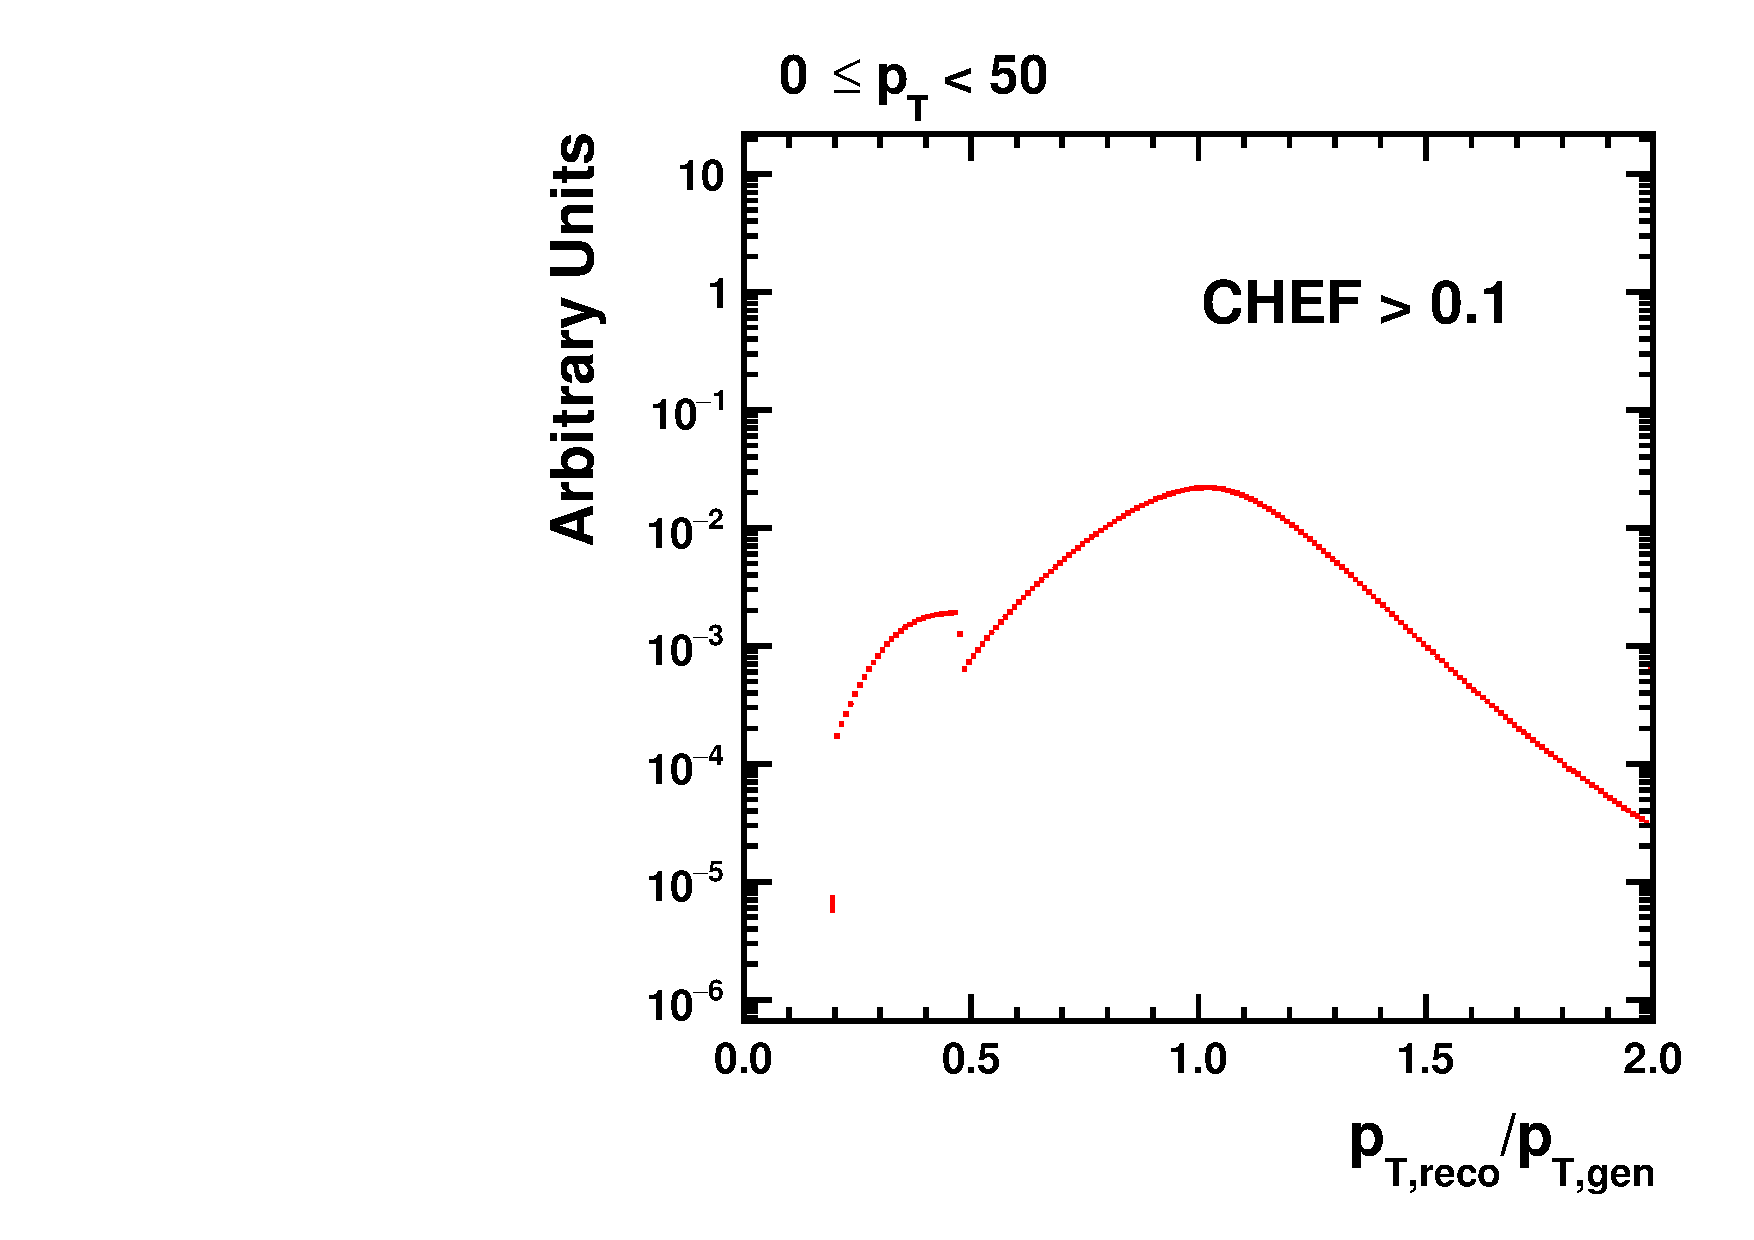
\includegraphics[width=0.25\textwidth]{diagnostics_NANO/res_light_NANO_1.pdf}
  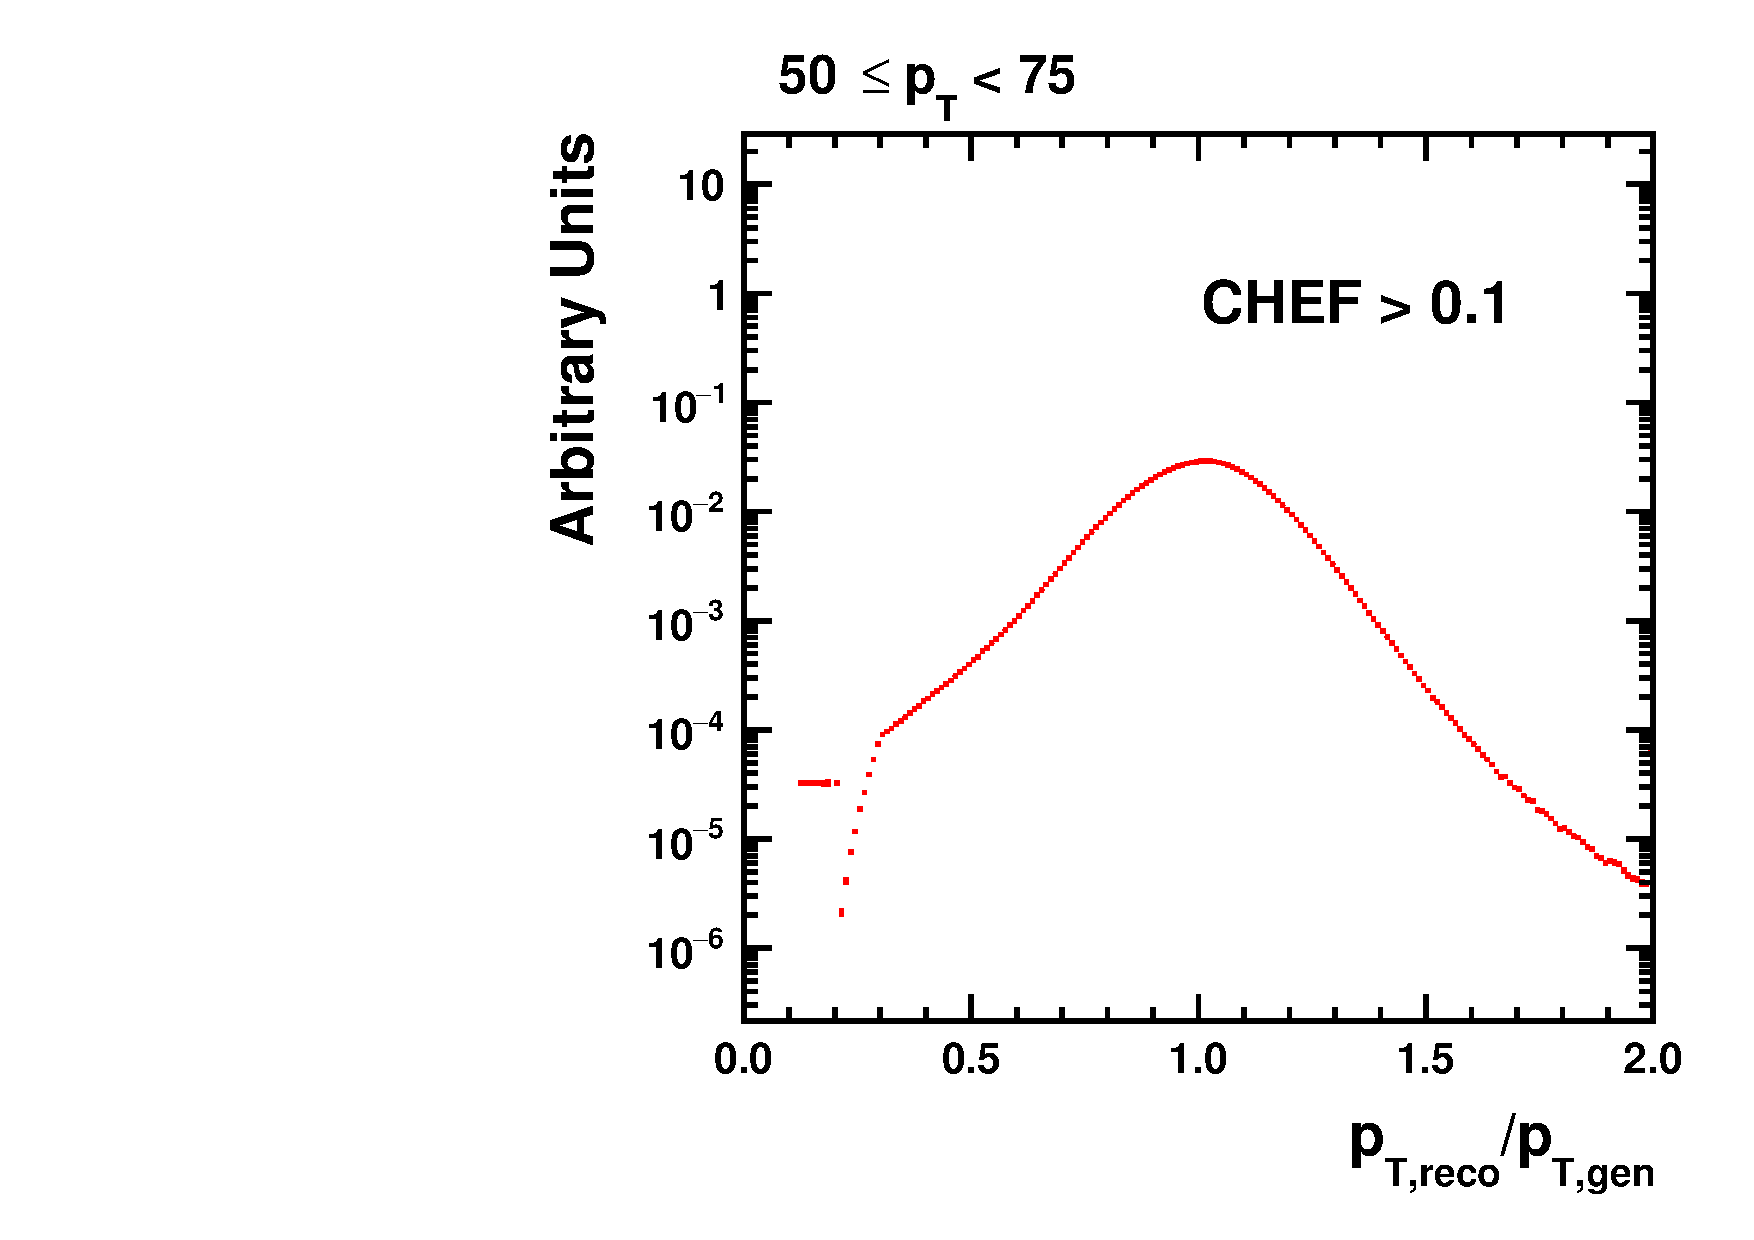
\includegraphics[width=0.25\textwidth]{diagnostics_NANO/res_light_NANO_2.pdf} 
  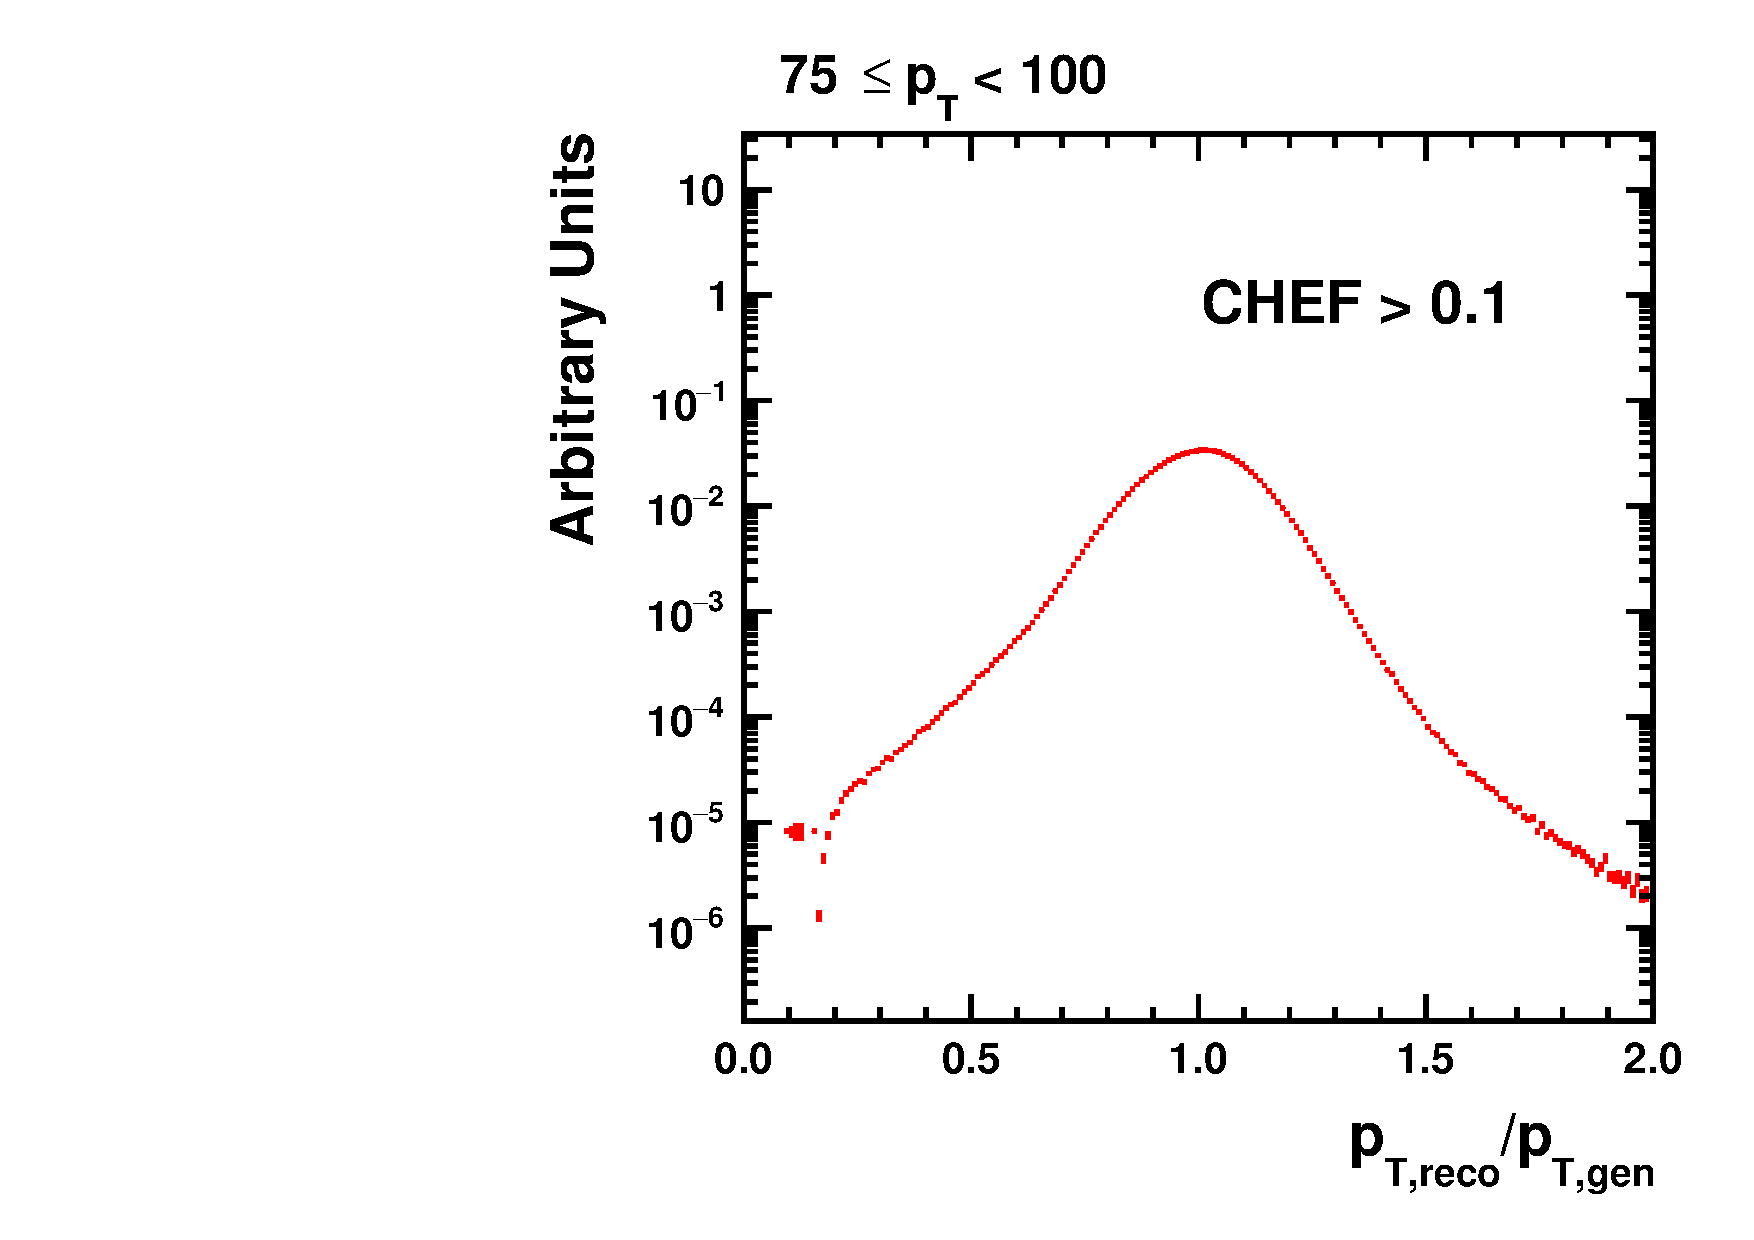
\includegraphics[width=0.25\textwidth]{diagnostics_NANO/res_light_NANO_3.pdf} \\
  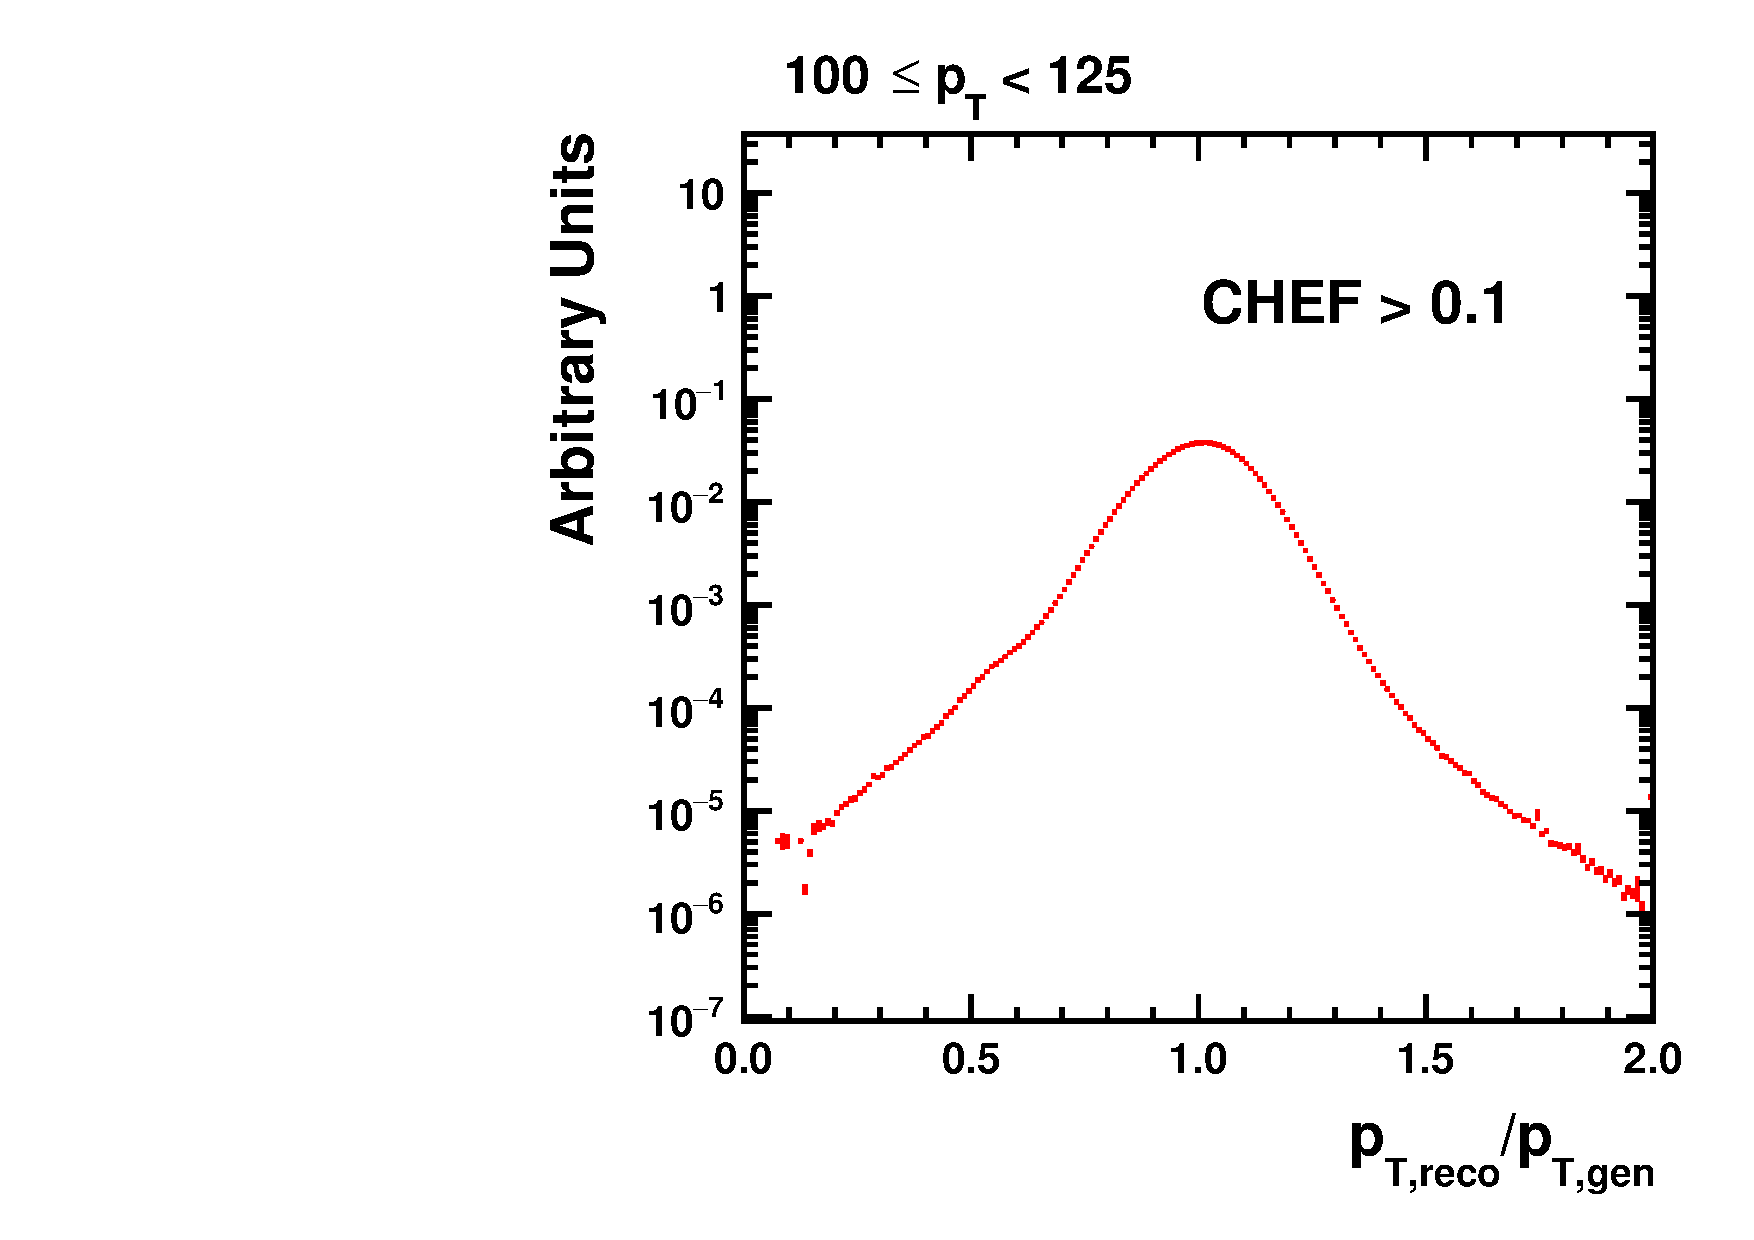
\includegraphics[width=0.25\textwidth]{diagnostics_NANO/res_light_NANO_4.pdf}
  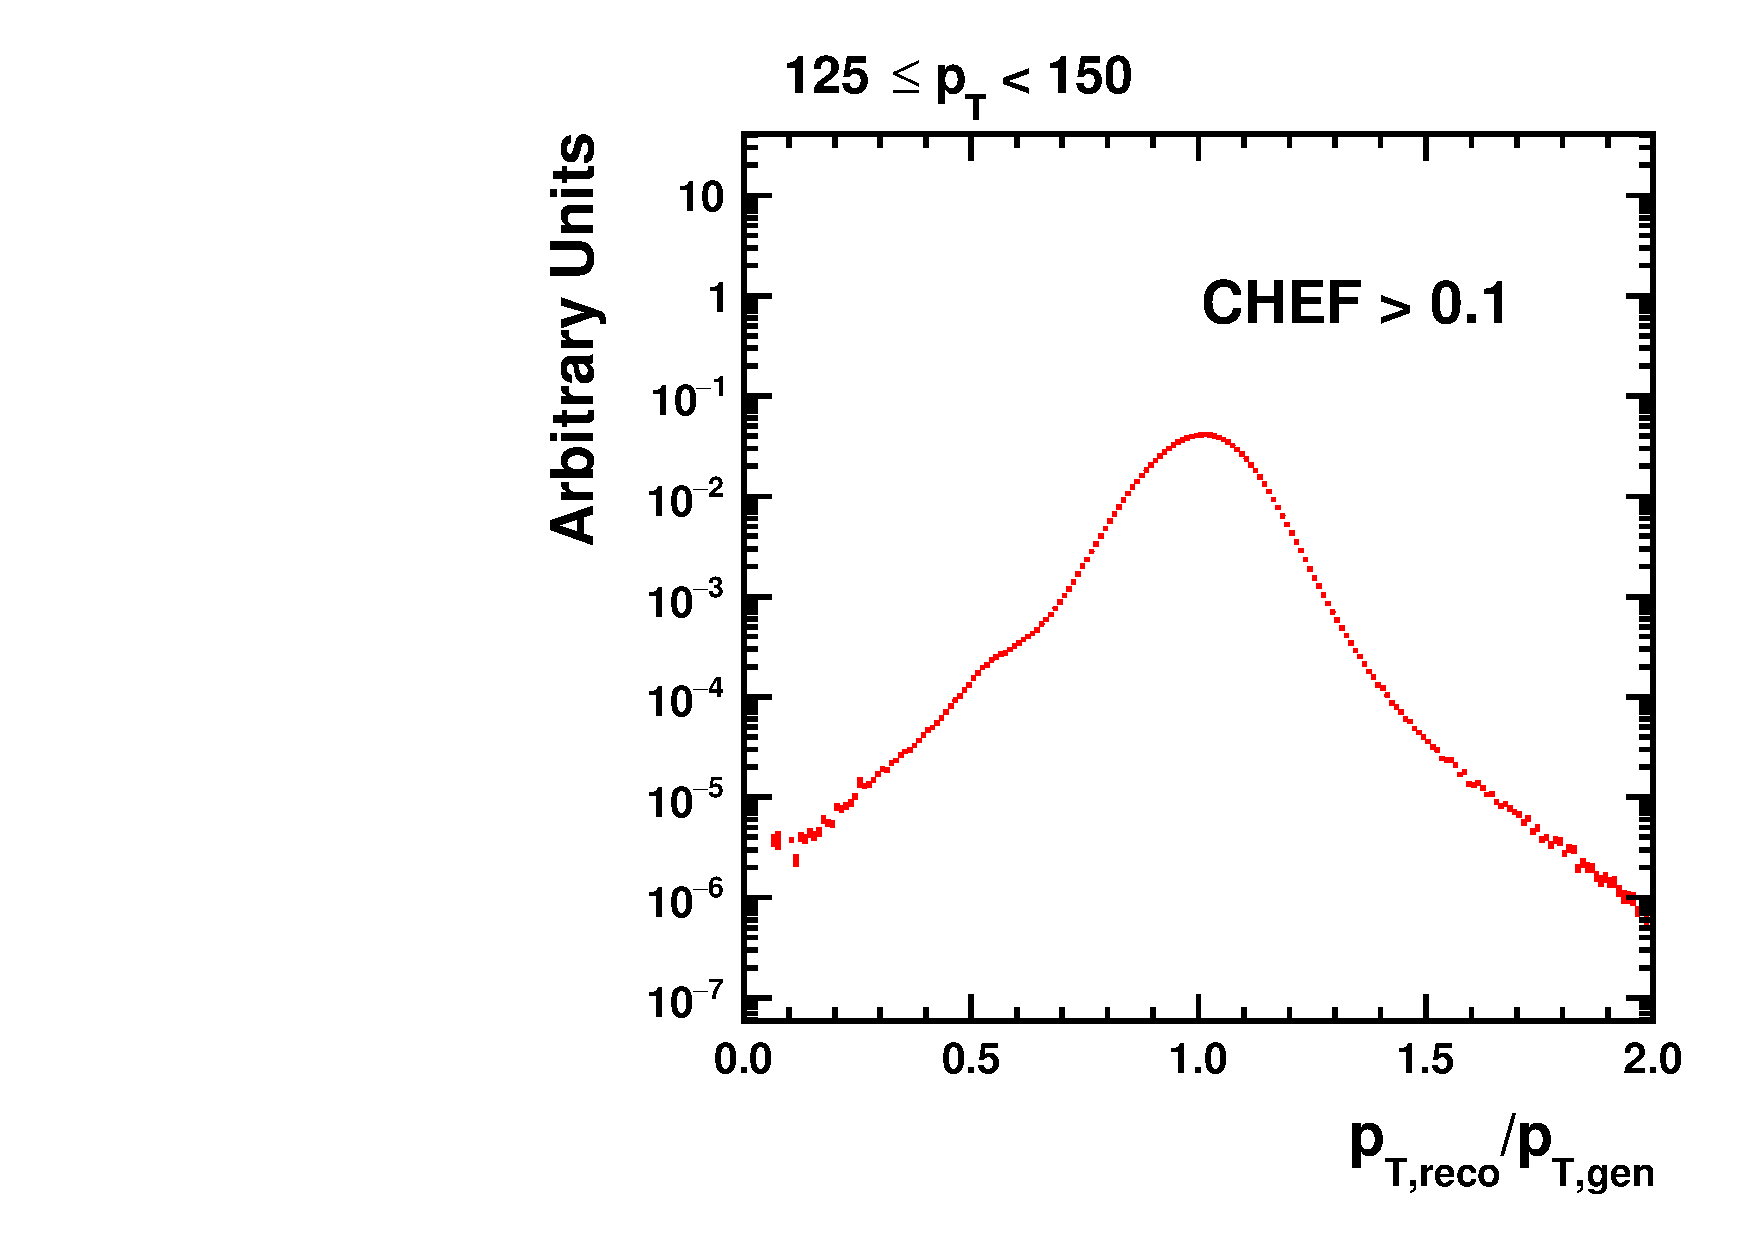
\includegraphics[width=0.25\textwidth]{diagnostics_NANO/res_light_NANO_5.pdf} 
  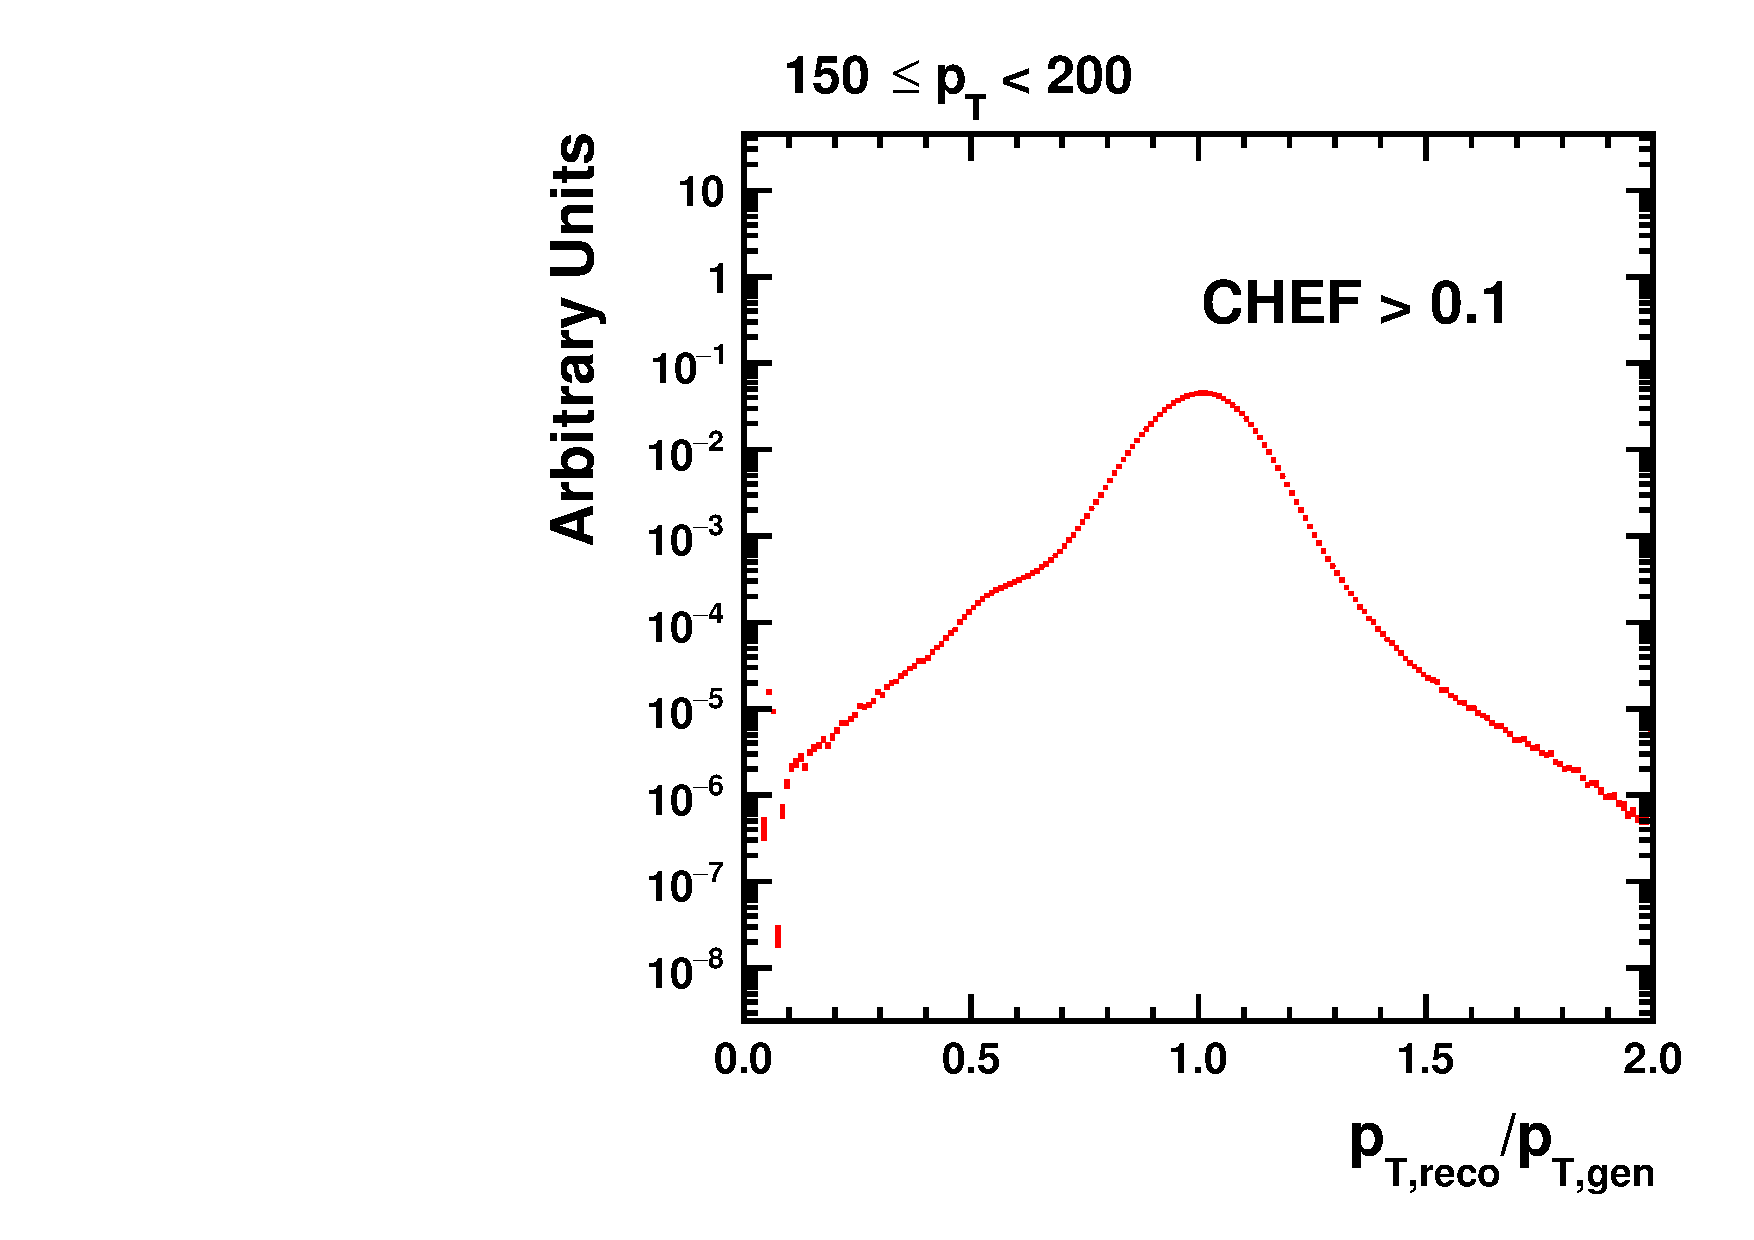
\includegraphics[width=0.25\textwidth]{diagnostics_NANO/res_light_NANO_6.pdf} \\
  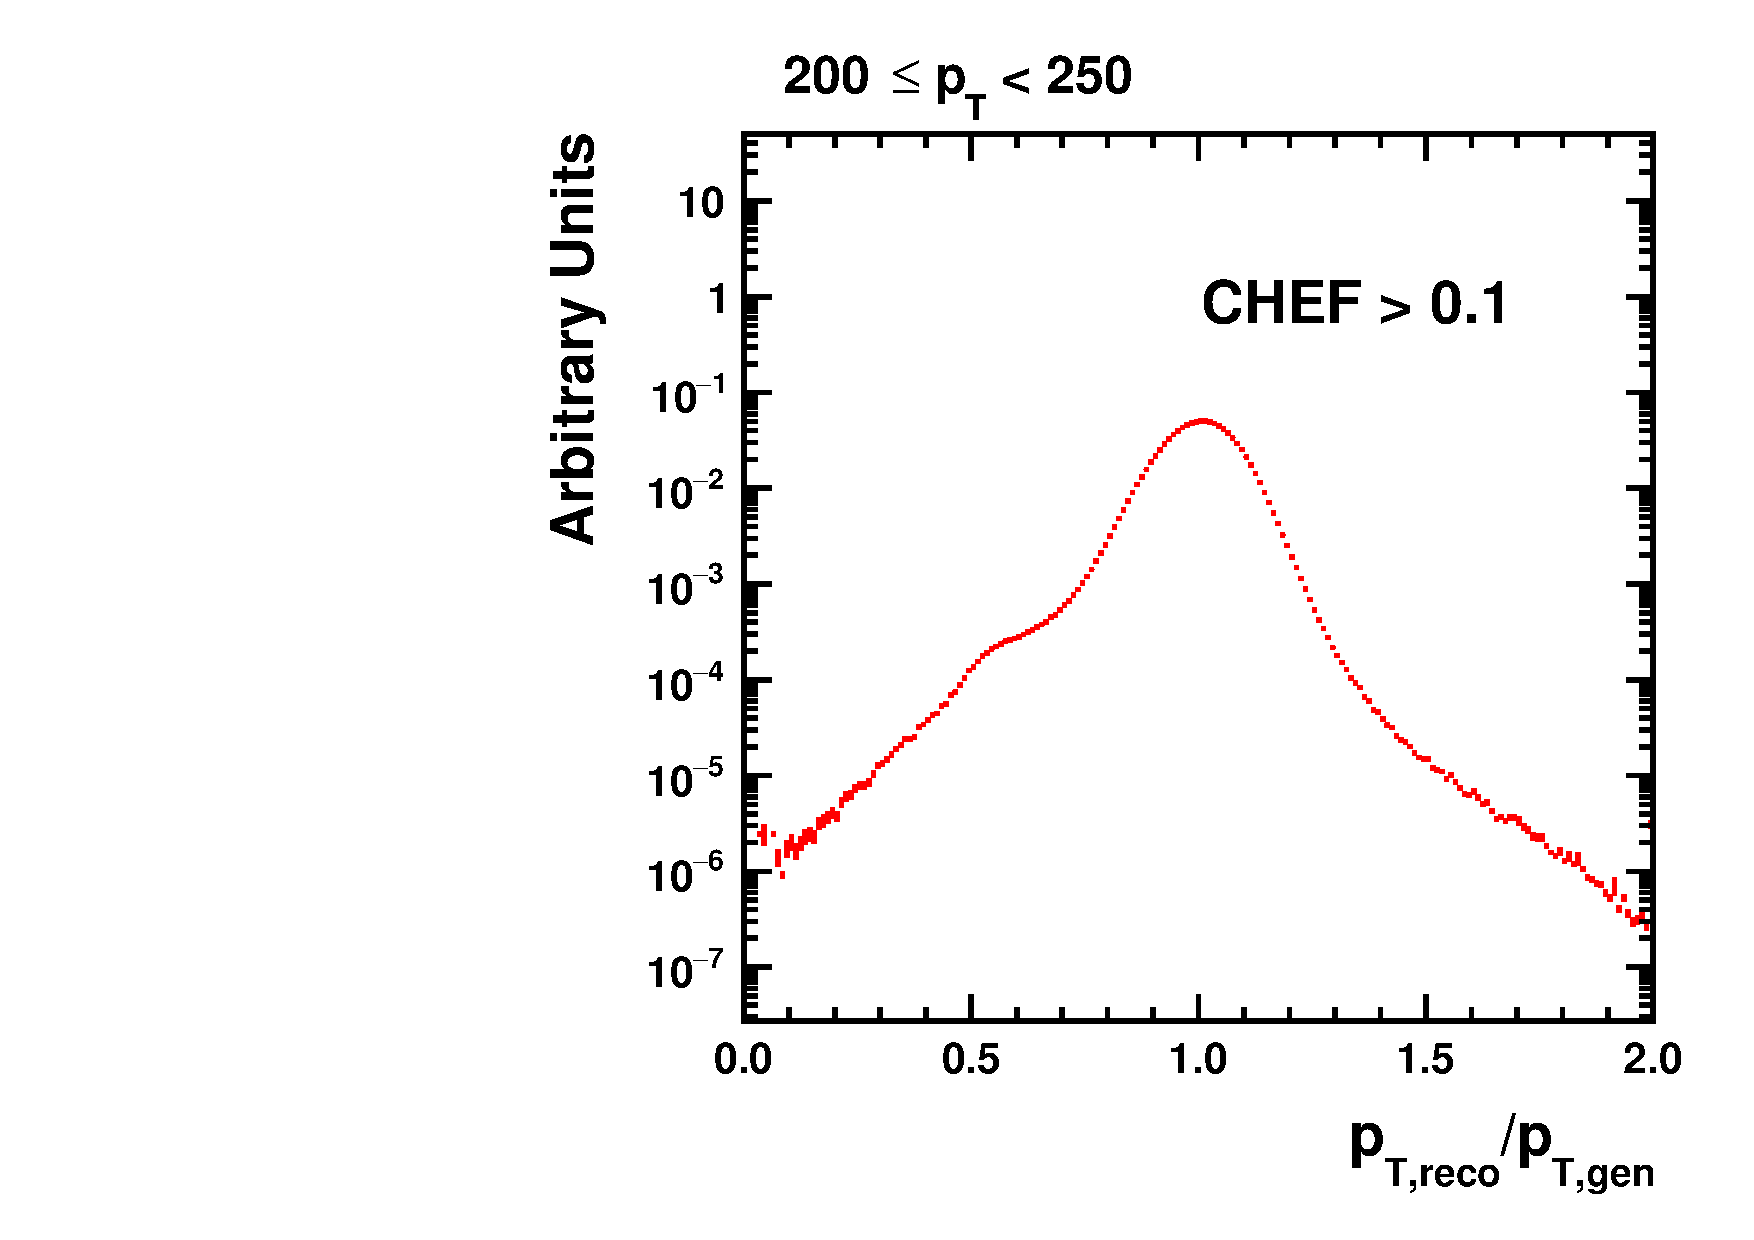
\includegraphics[width=0.25\textwidth]{diagnostics_NANO/res_light_NANO_7.pdf}
  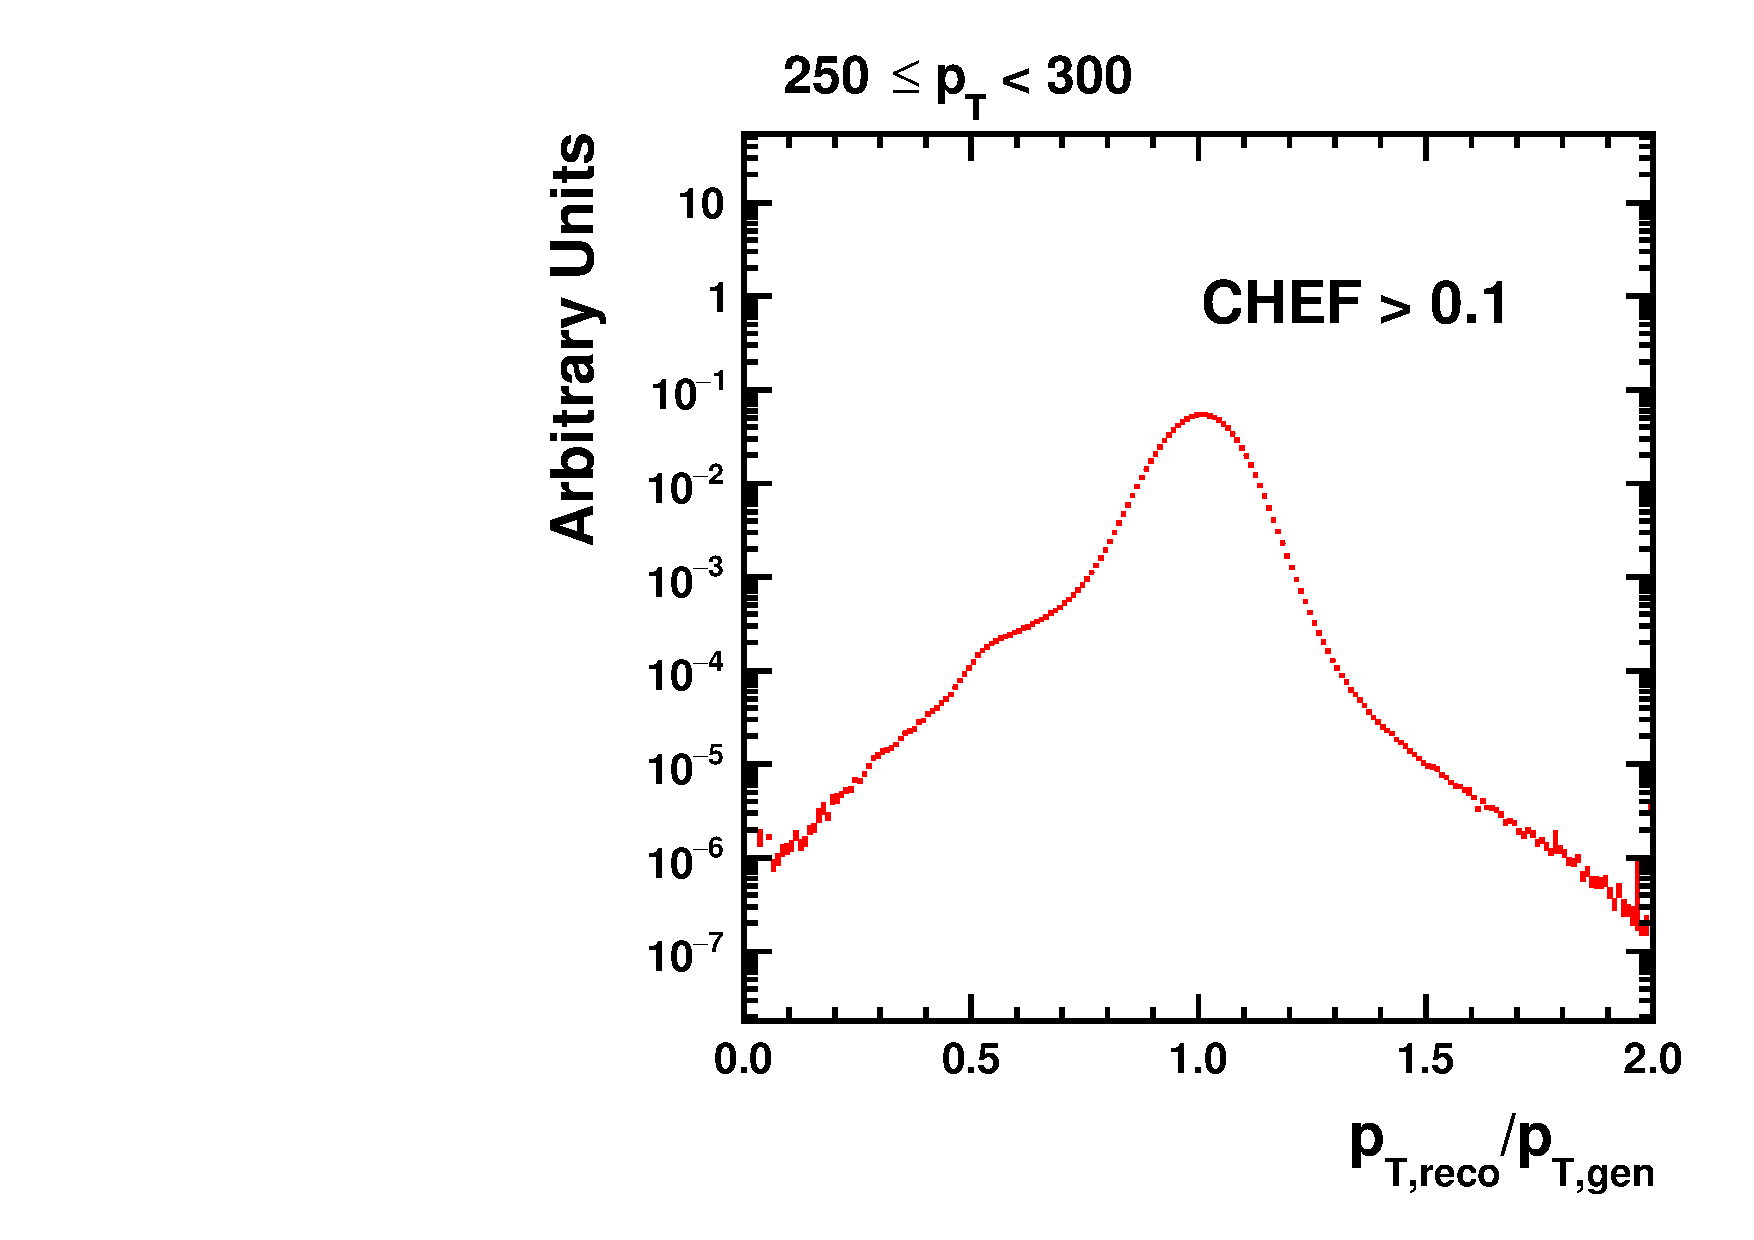
\includegraphics[width=0.25\textwidth]{diagnostics_NANO/res_light_NANO_8.pdf} 
  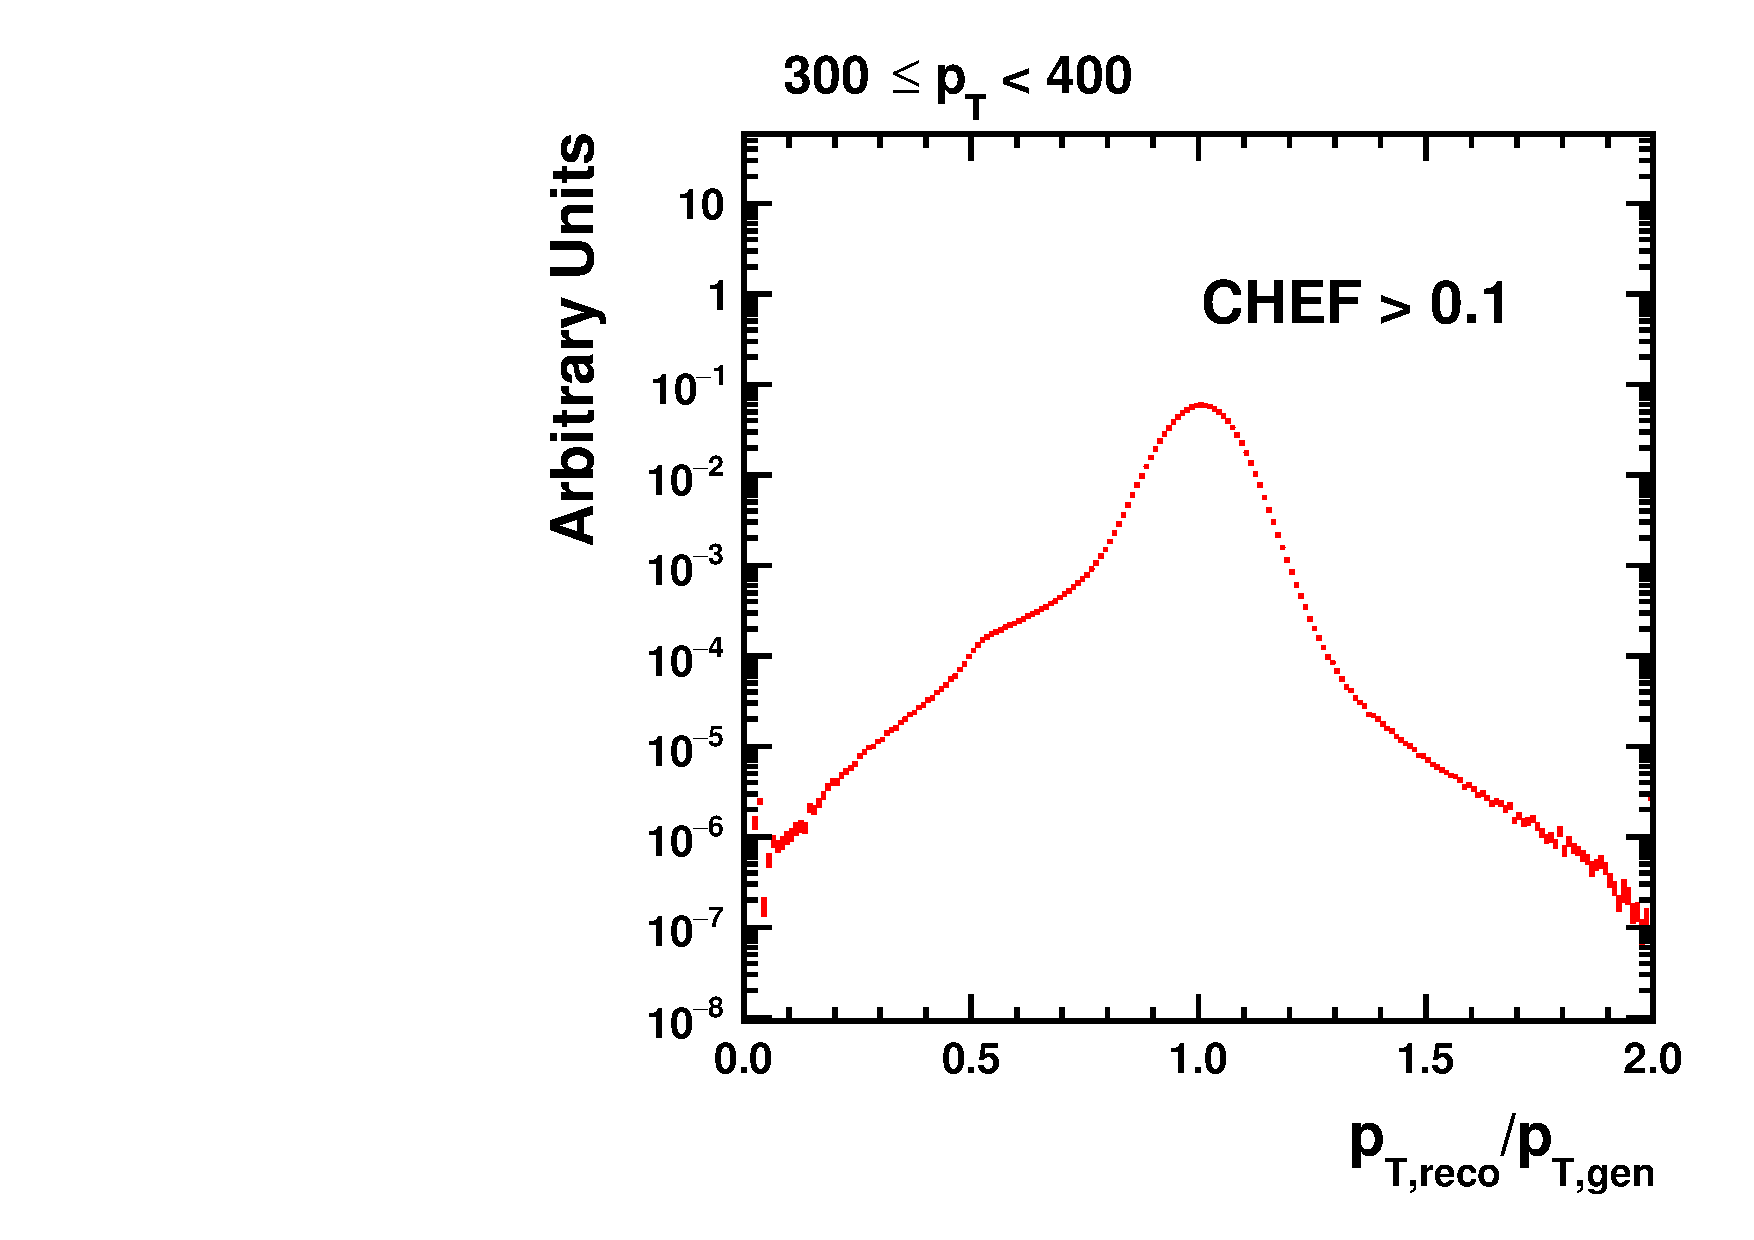
\includegraphics[width=0.25\textwidth]{diagnostics_NANO/res_light_NANO_9.pdf} \\
  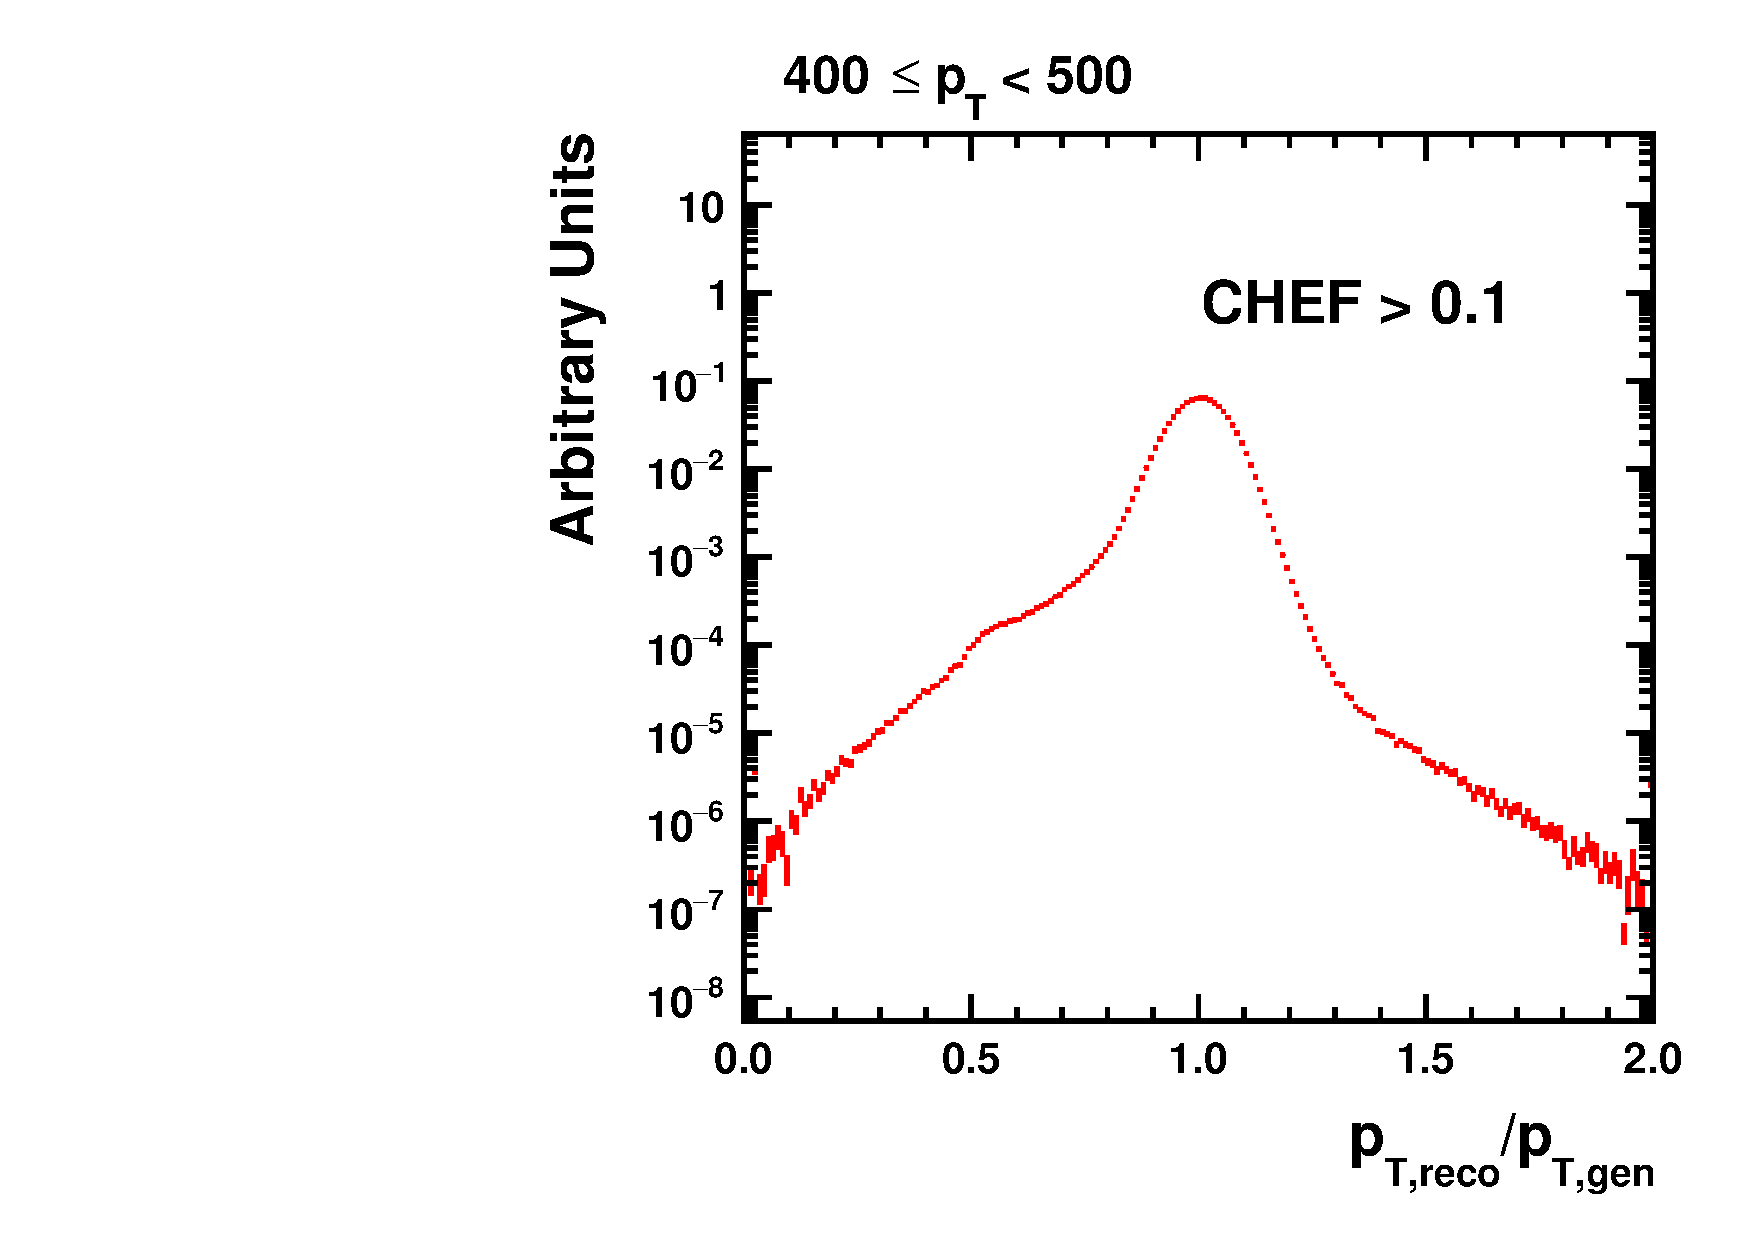
\includegraphics[width=0.25\textwidth]{diagnostics_NANO/res_light_NANO_10.pdf}
  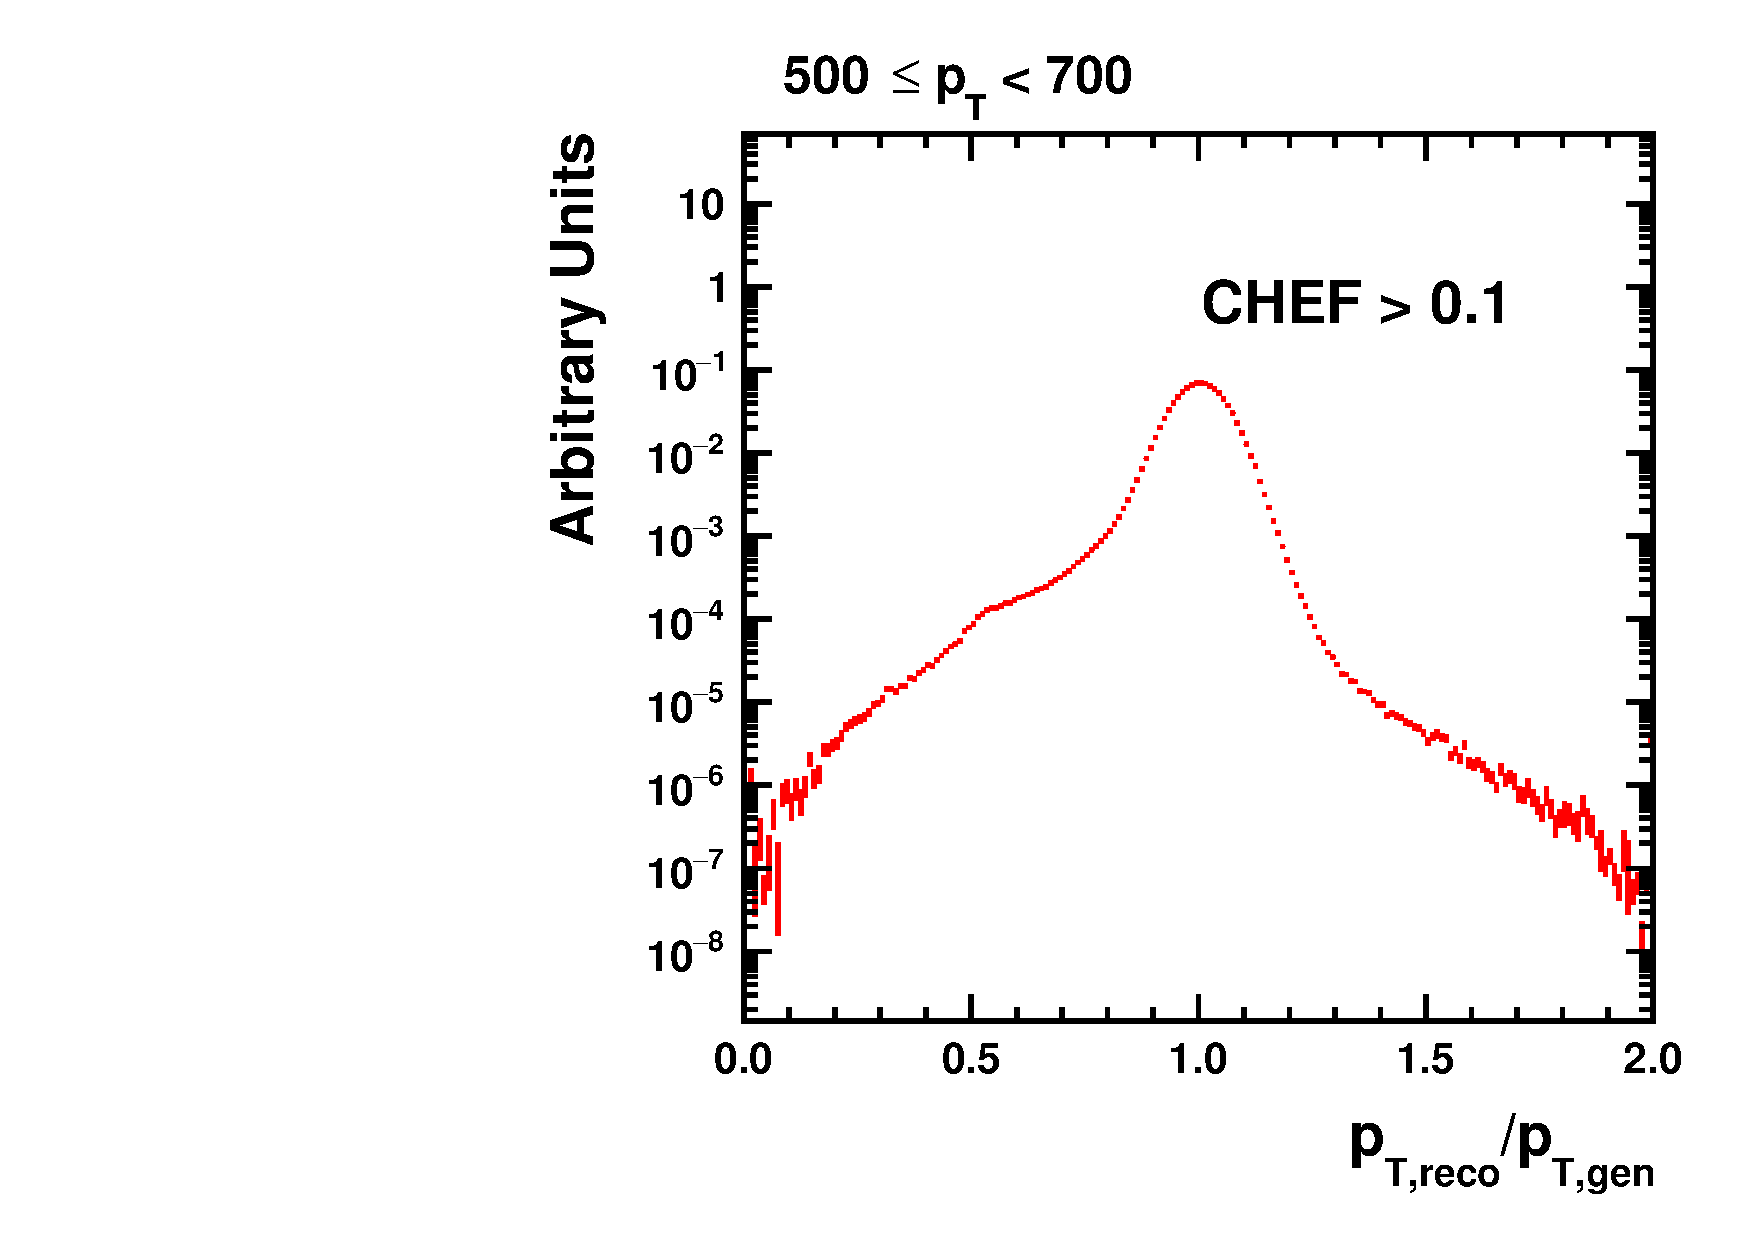
\includegraphics[width=0.25\textwidth]{diagnostics_NANO/res_light_NANO_11.pdf} 
  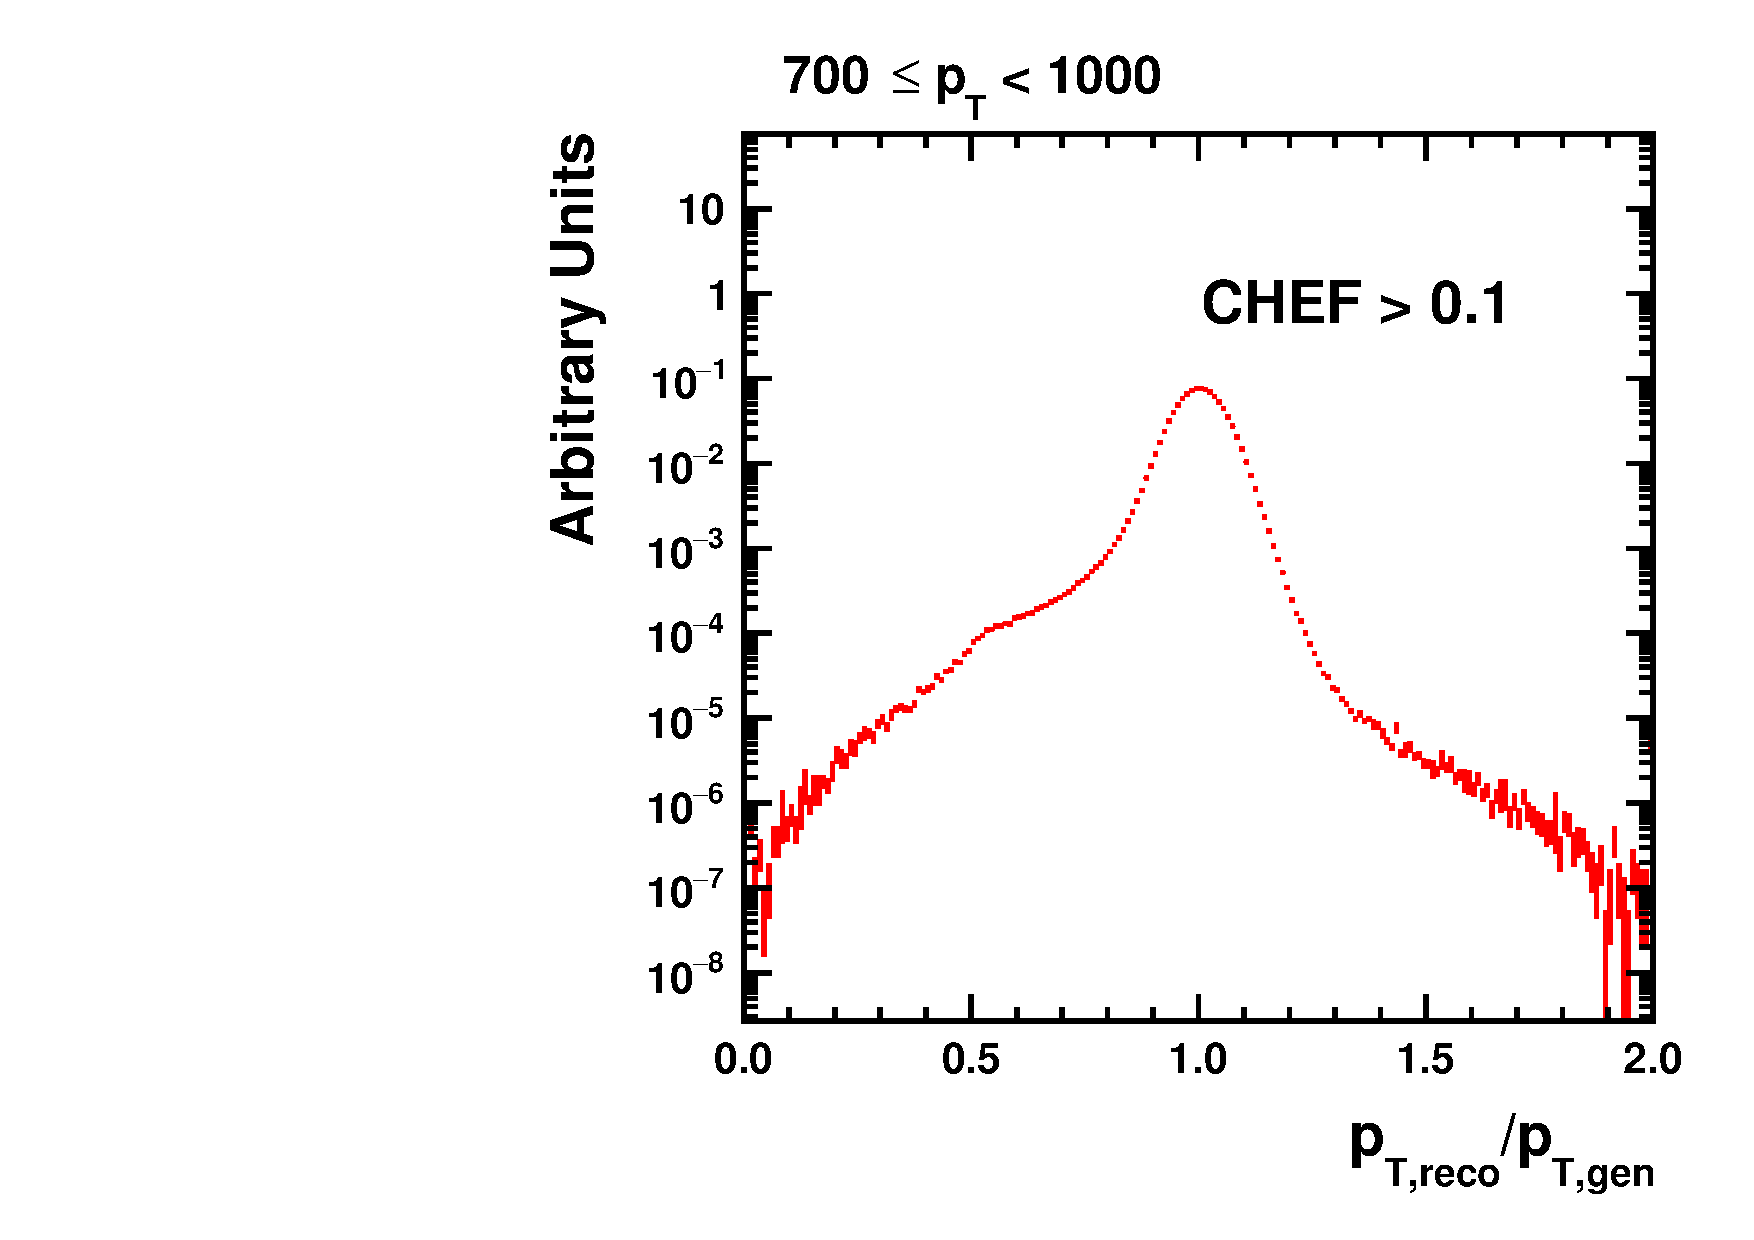
\includegraphics[width=0.25\textwidth]{diagnostics_NANO/res_light_NANO_12.pdf}     
  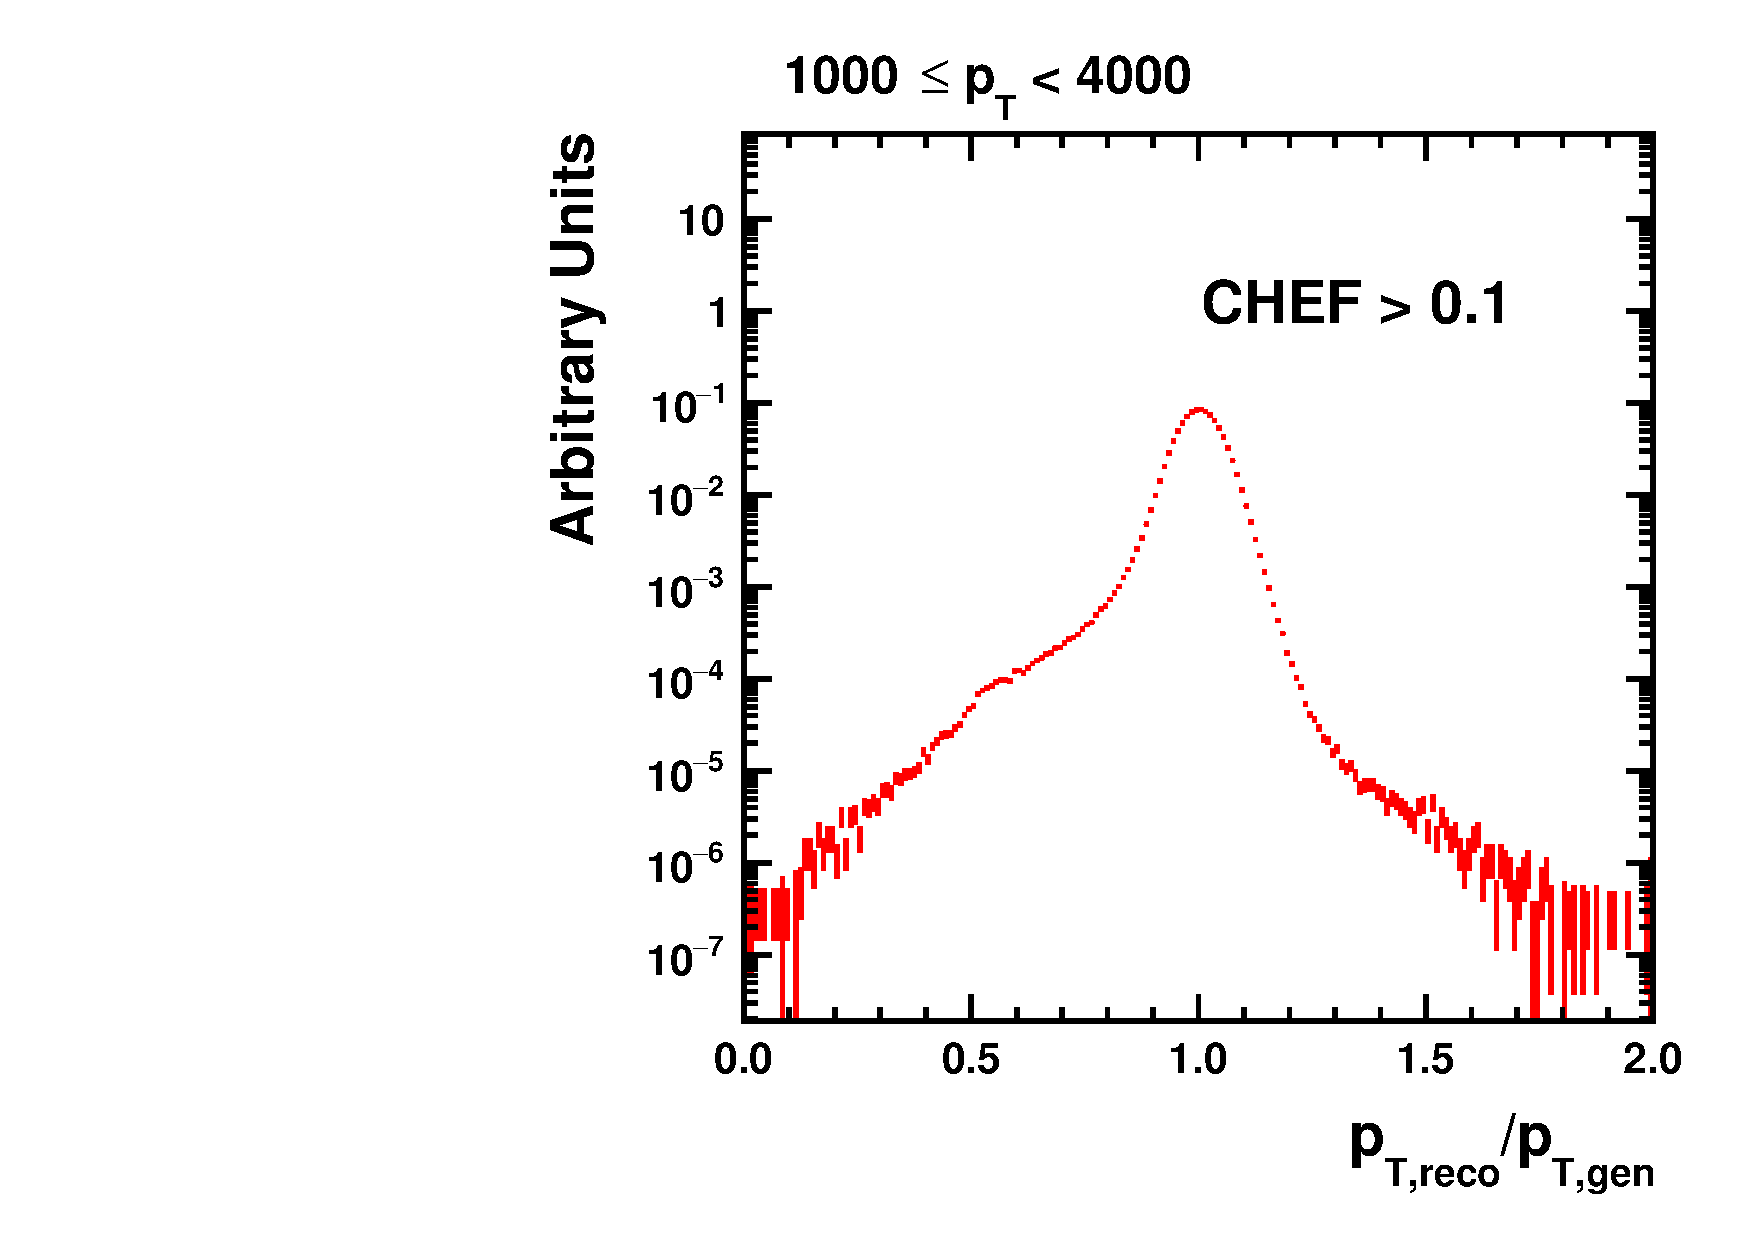
\includegraphics[width=0.25\textwidth]{diagnostics_NANO/res_light_NANO_13.pdf} \\      
	\end{center}
	\caption[Light Jet Response]{Comparison of the Data and MC in the 1Lep CR for each era: Run2016, Run2017BtoE, Run2017F, Run2018preHEM, Run2018PostHEM, and the combination of all eras in the Low \dm{} region. Each era has a good agreement between Data and MC. 
	 }
	\label{fig:qcd-1lcr-datavsmc-lm-inclusive}
\end{figure}
\begin{figure}[!htb]
	\begin{center}  
  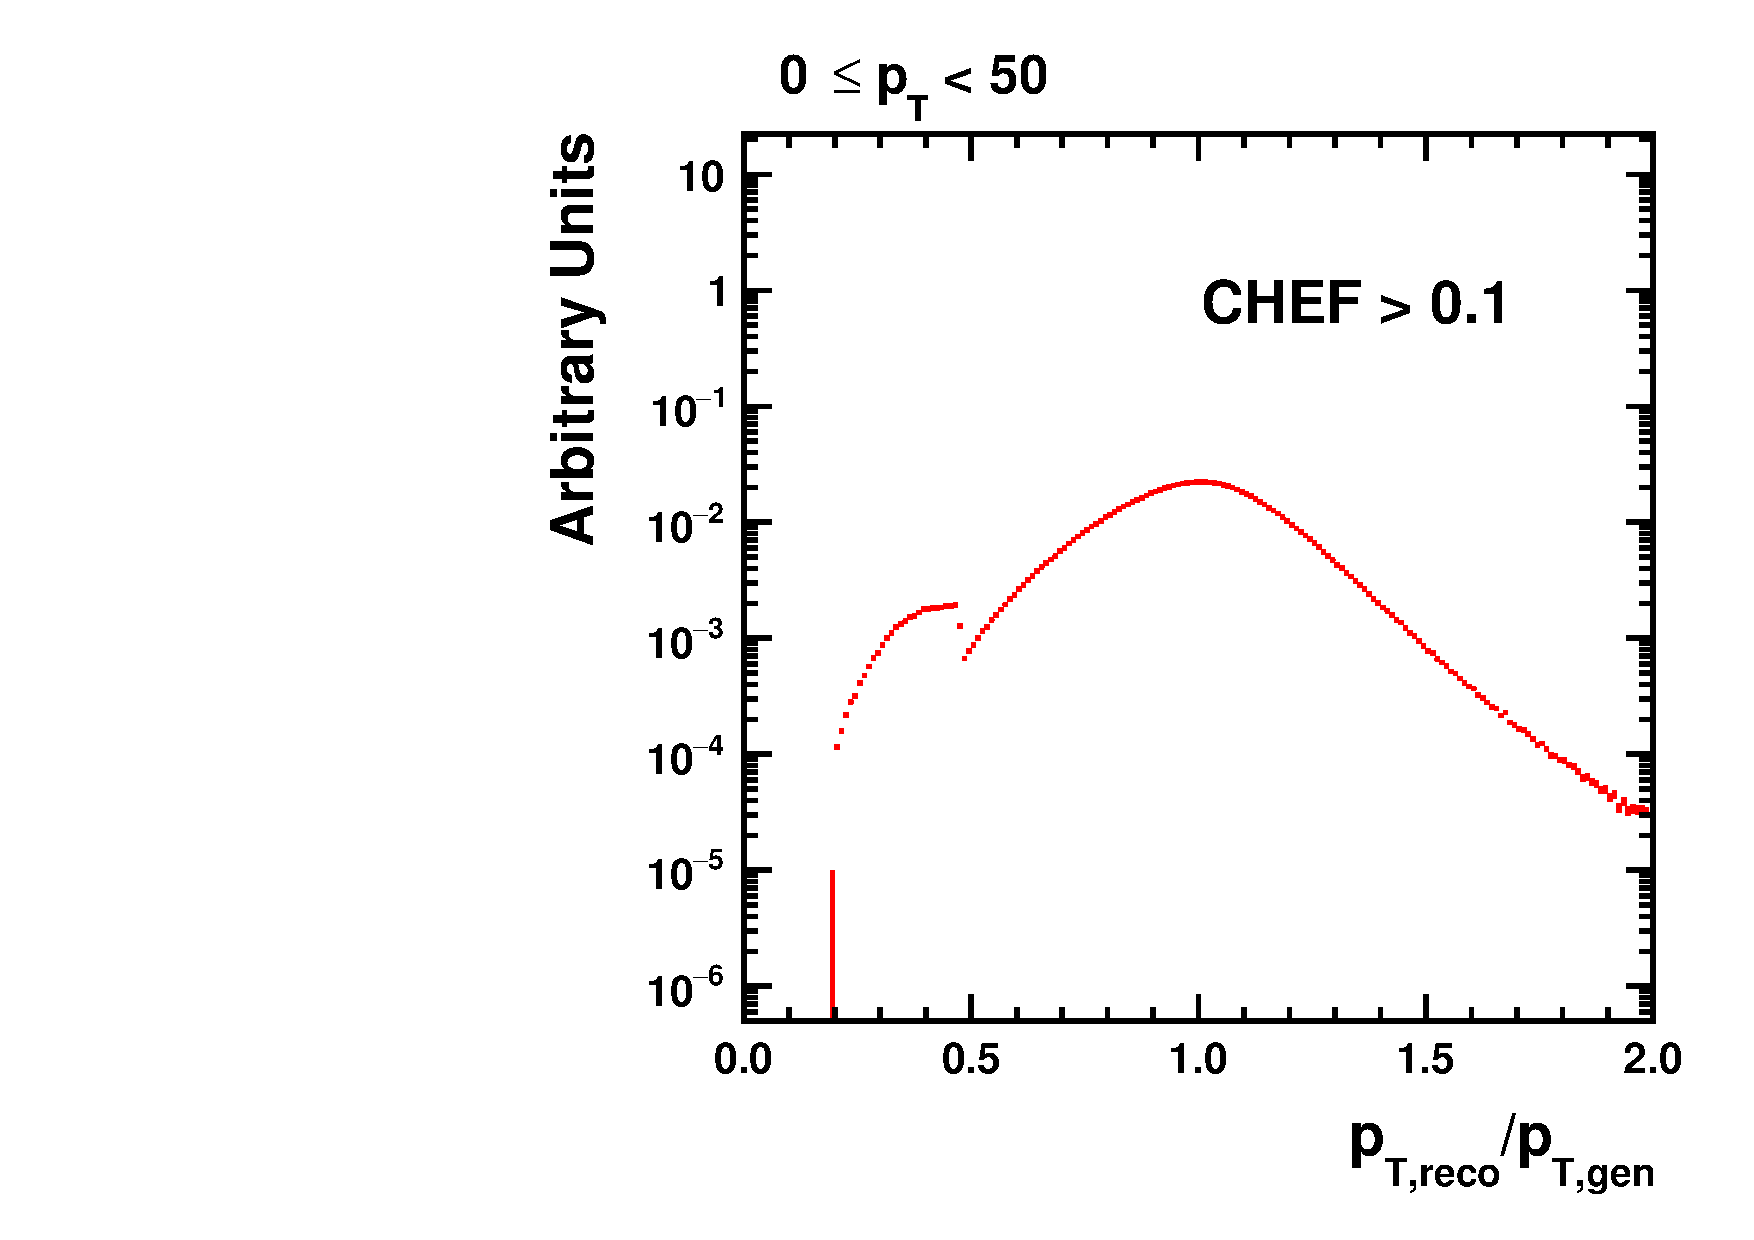
\includegraphics[width=0.25\textwidth]{diagnostics_NANO/res_b_NANO_1.pdf}
  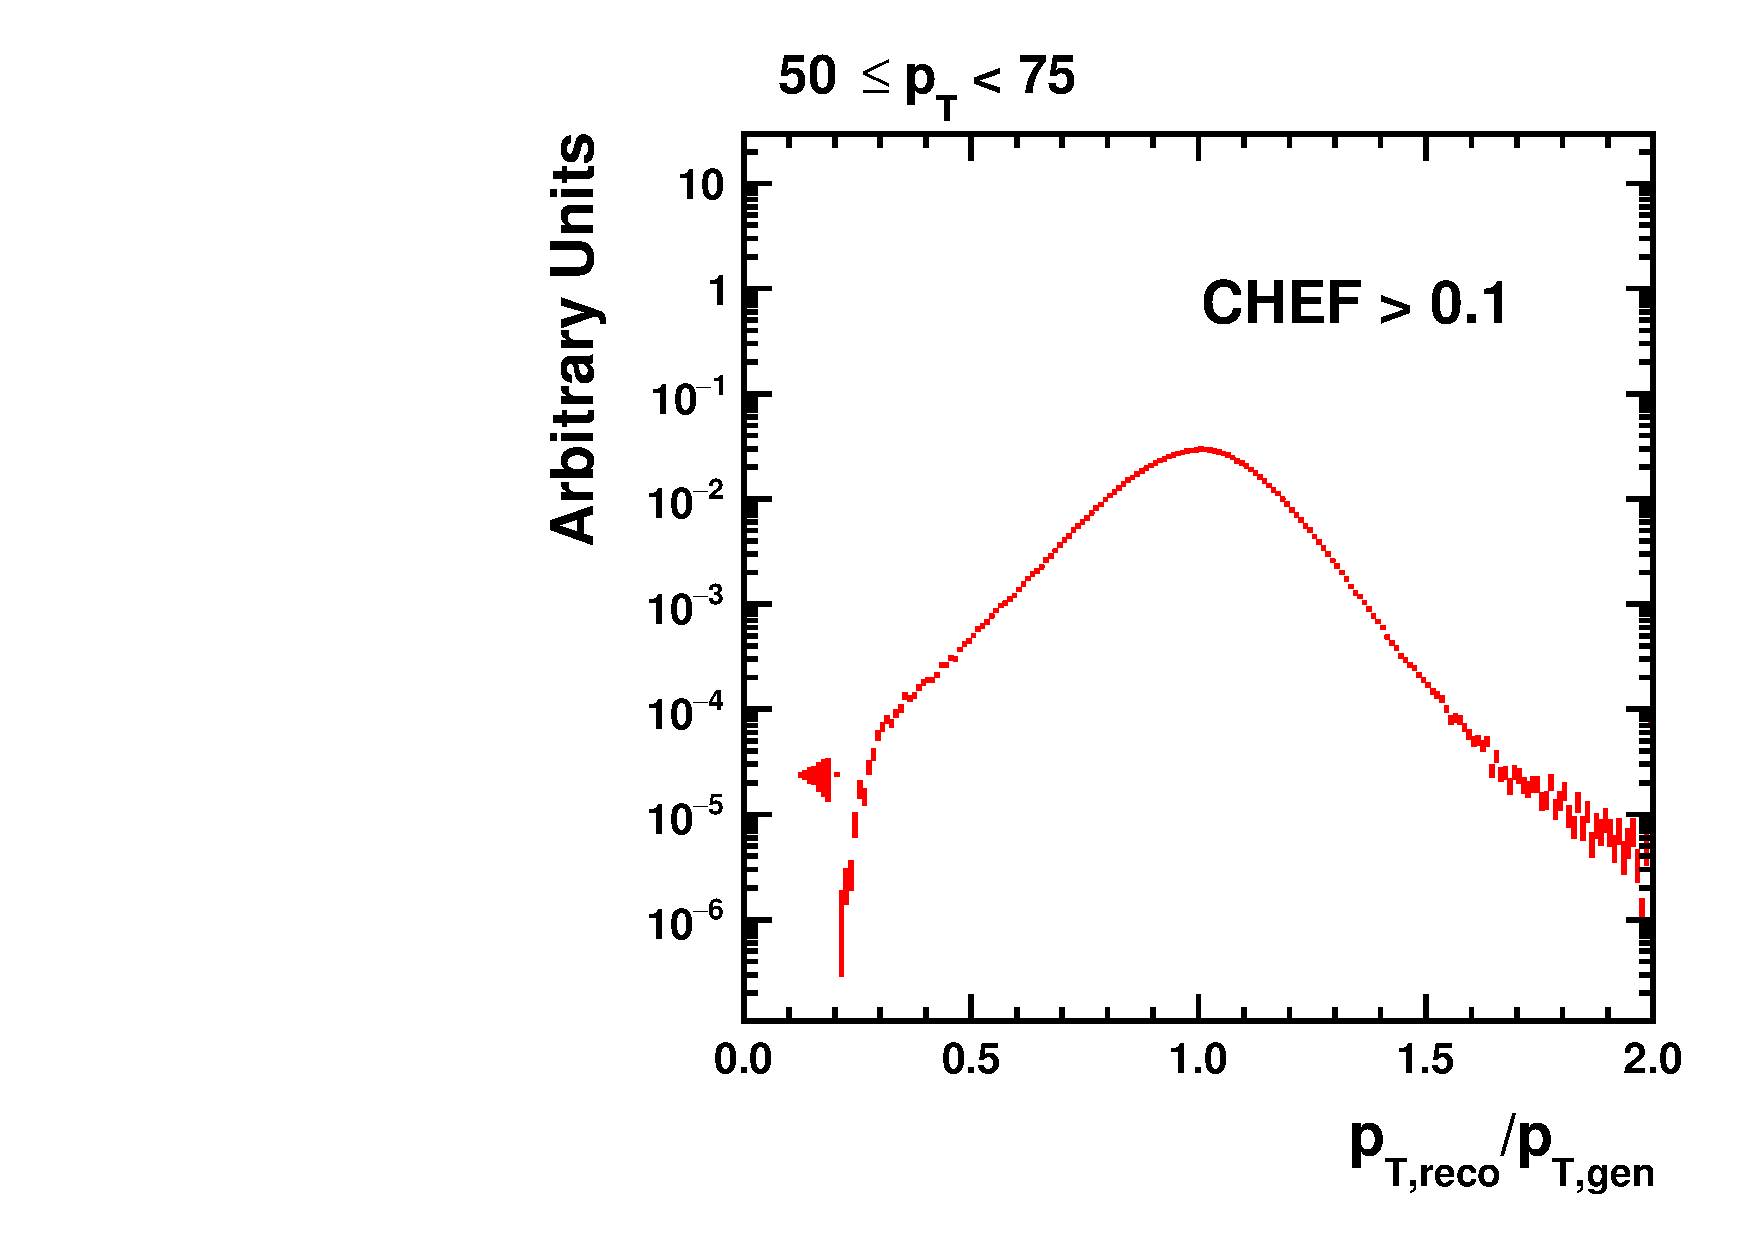
\includegraphics[width=0.25\textwidth]{diagnostics_NANO/res_b_NANO_2.pdf} 
  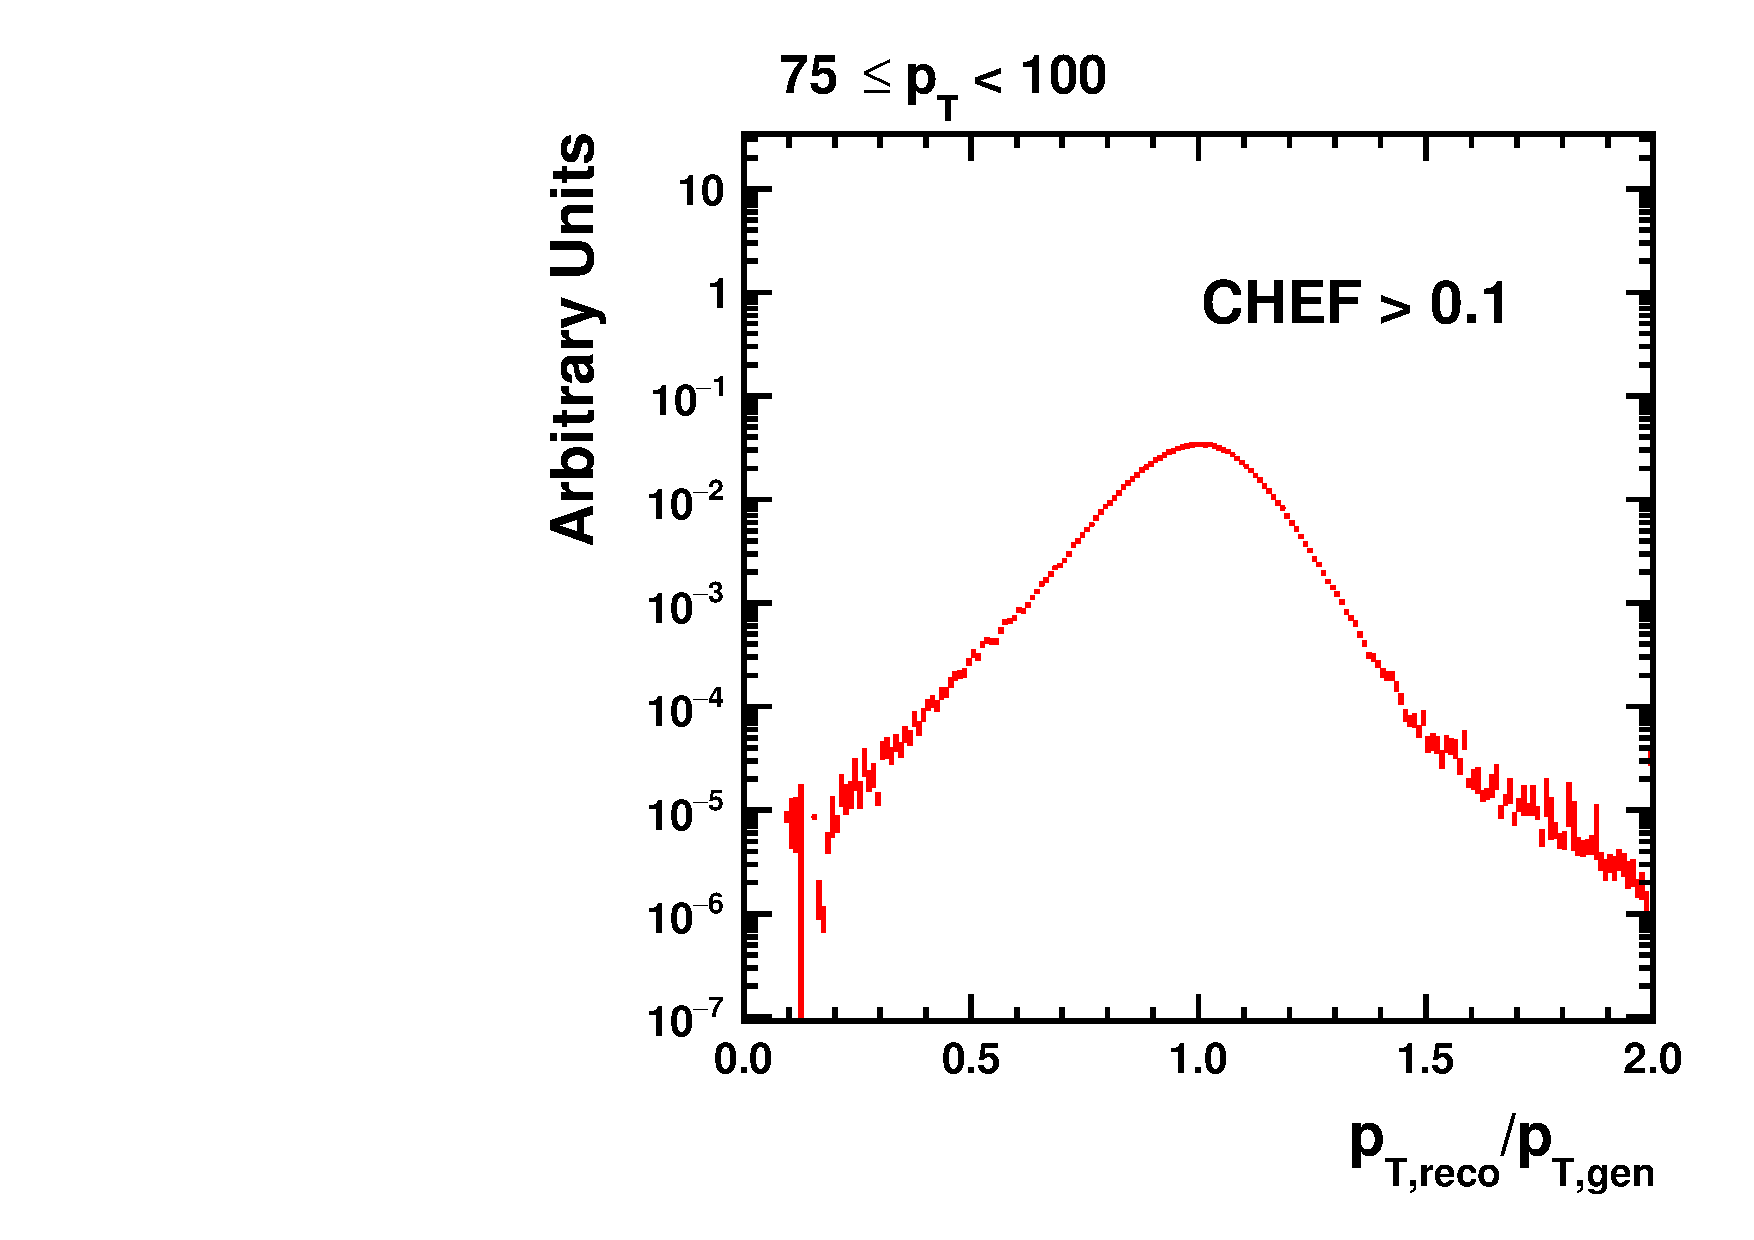
\includegraphics[width=0.25\textwidth]{diagnostics_NANO/res_b_NANO_3.pdf} \\
  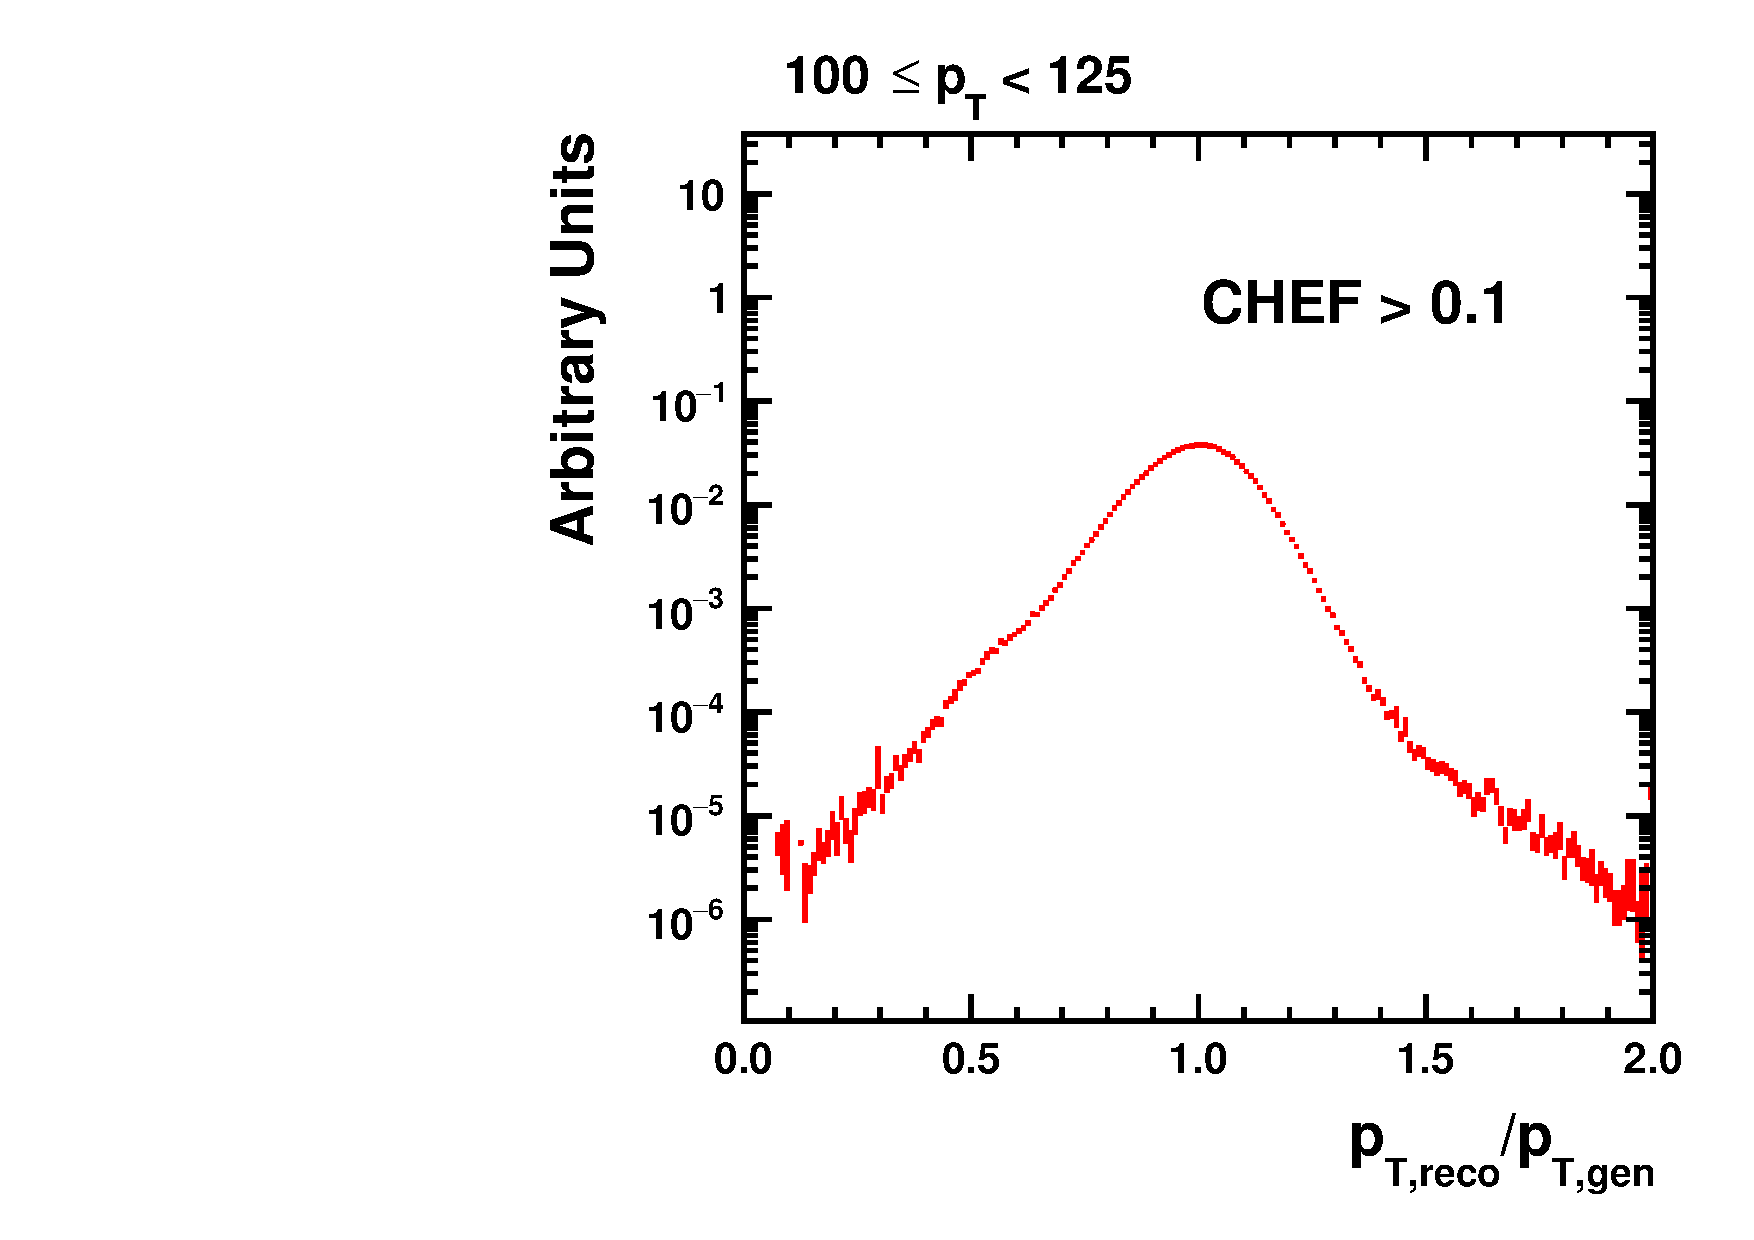
\includegraphics[width=0.25\textwidth]{diagnostics_NANO/res_b_NANO_4.pdf}
  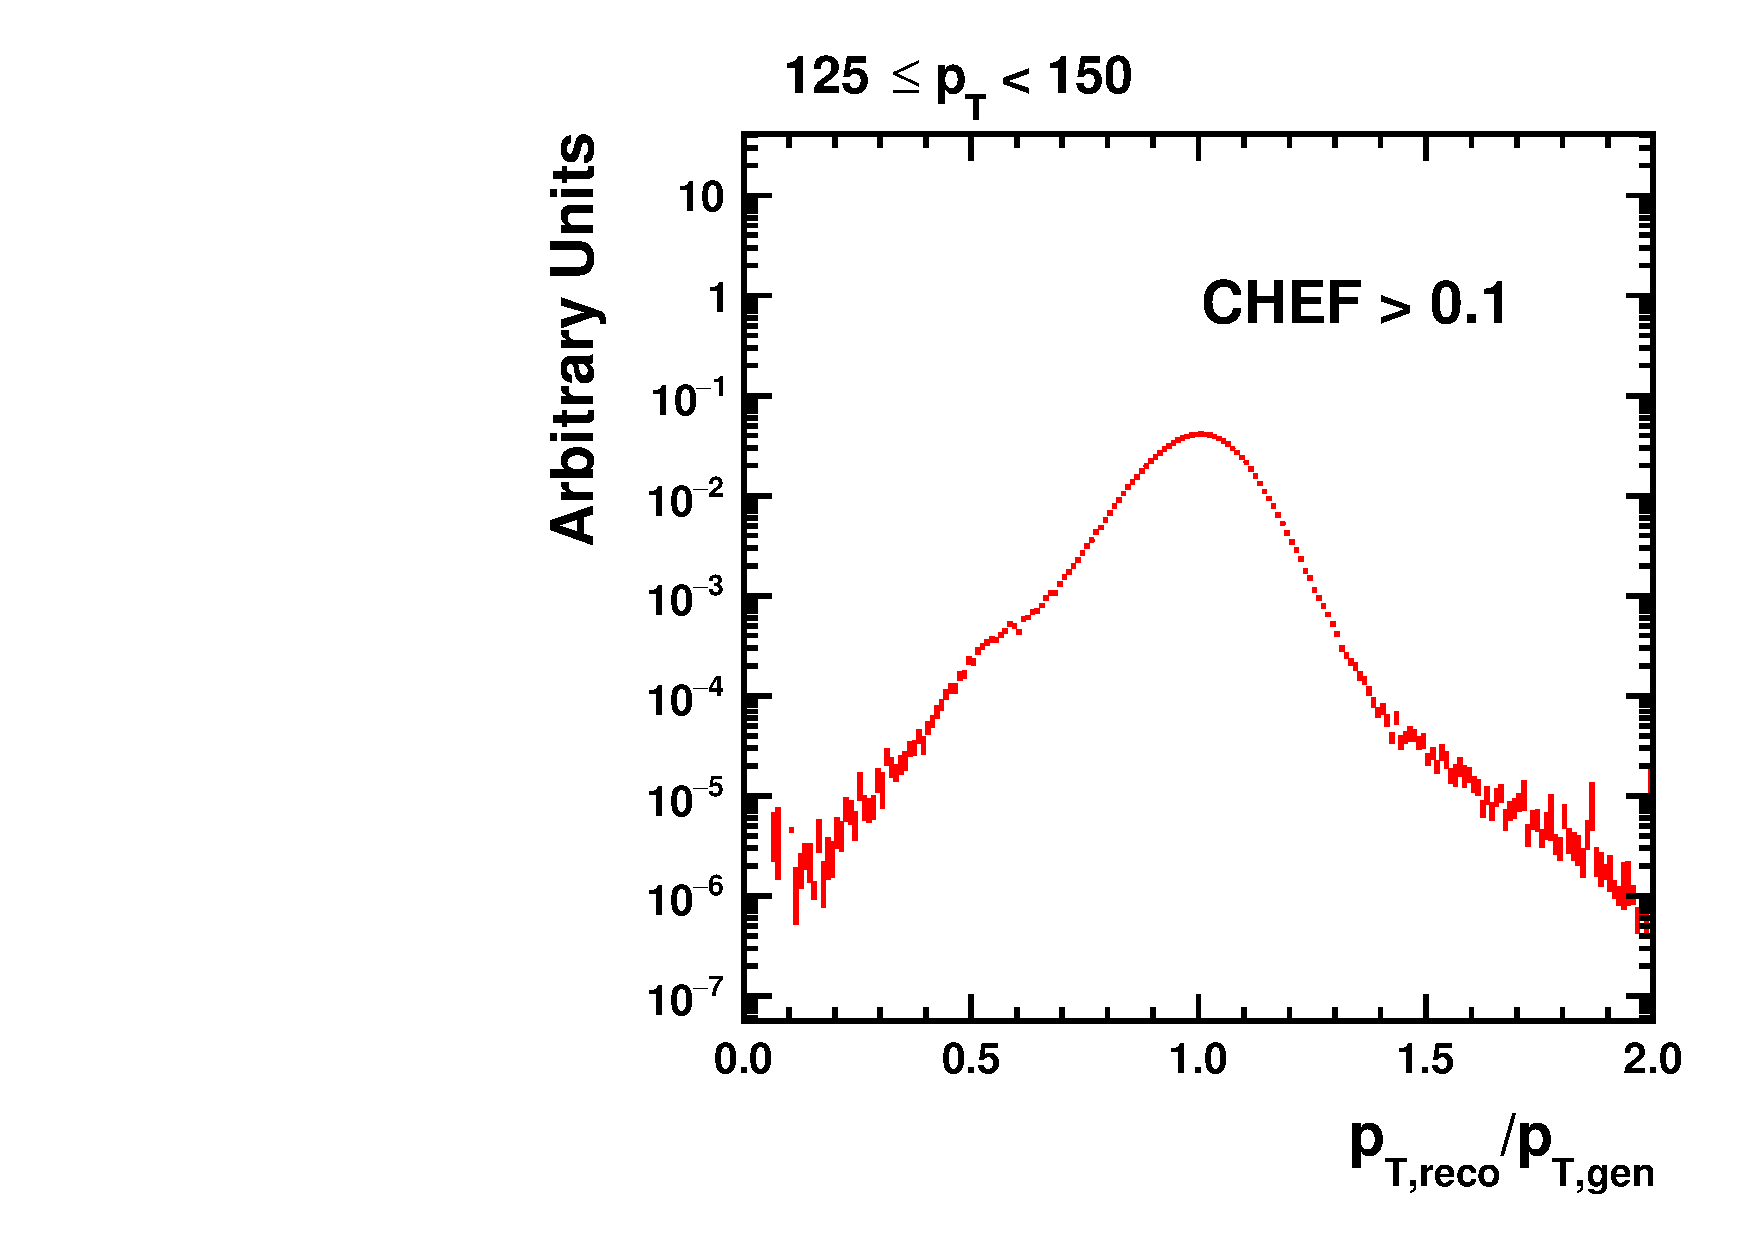
\includegraphics[width=0.25\textwidth]{diagnostics_NANO/res_b_NANO_5.pdf} 
  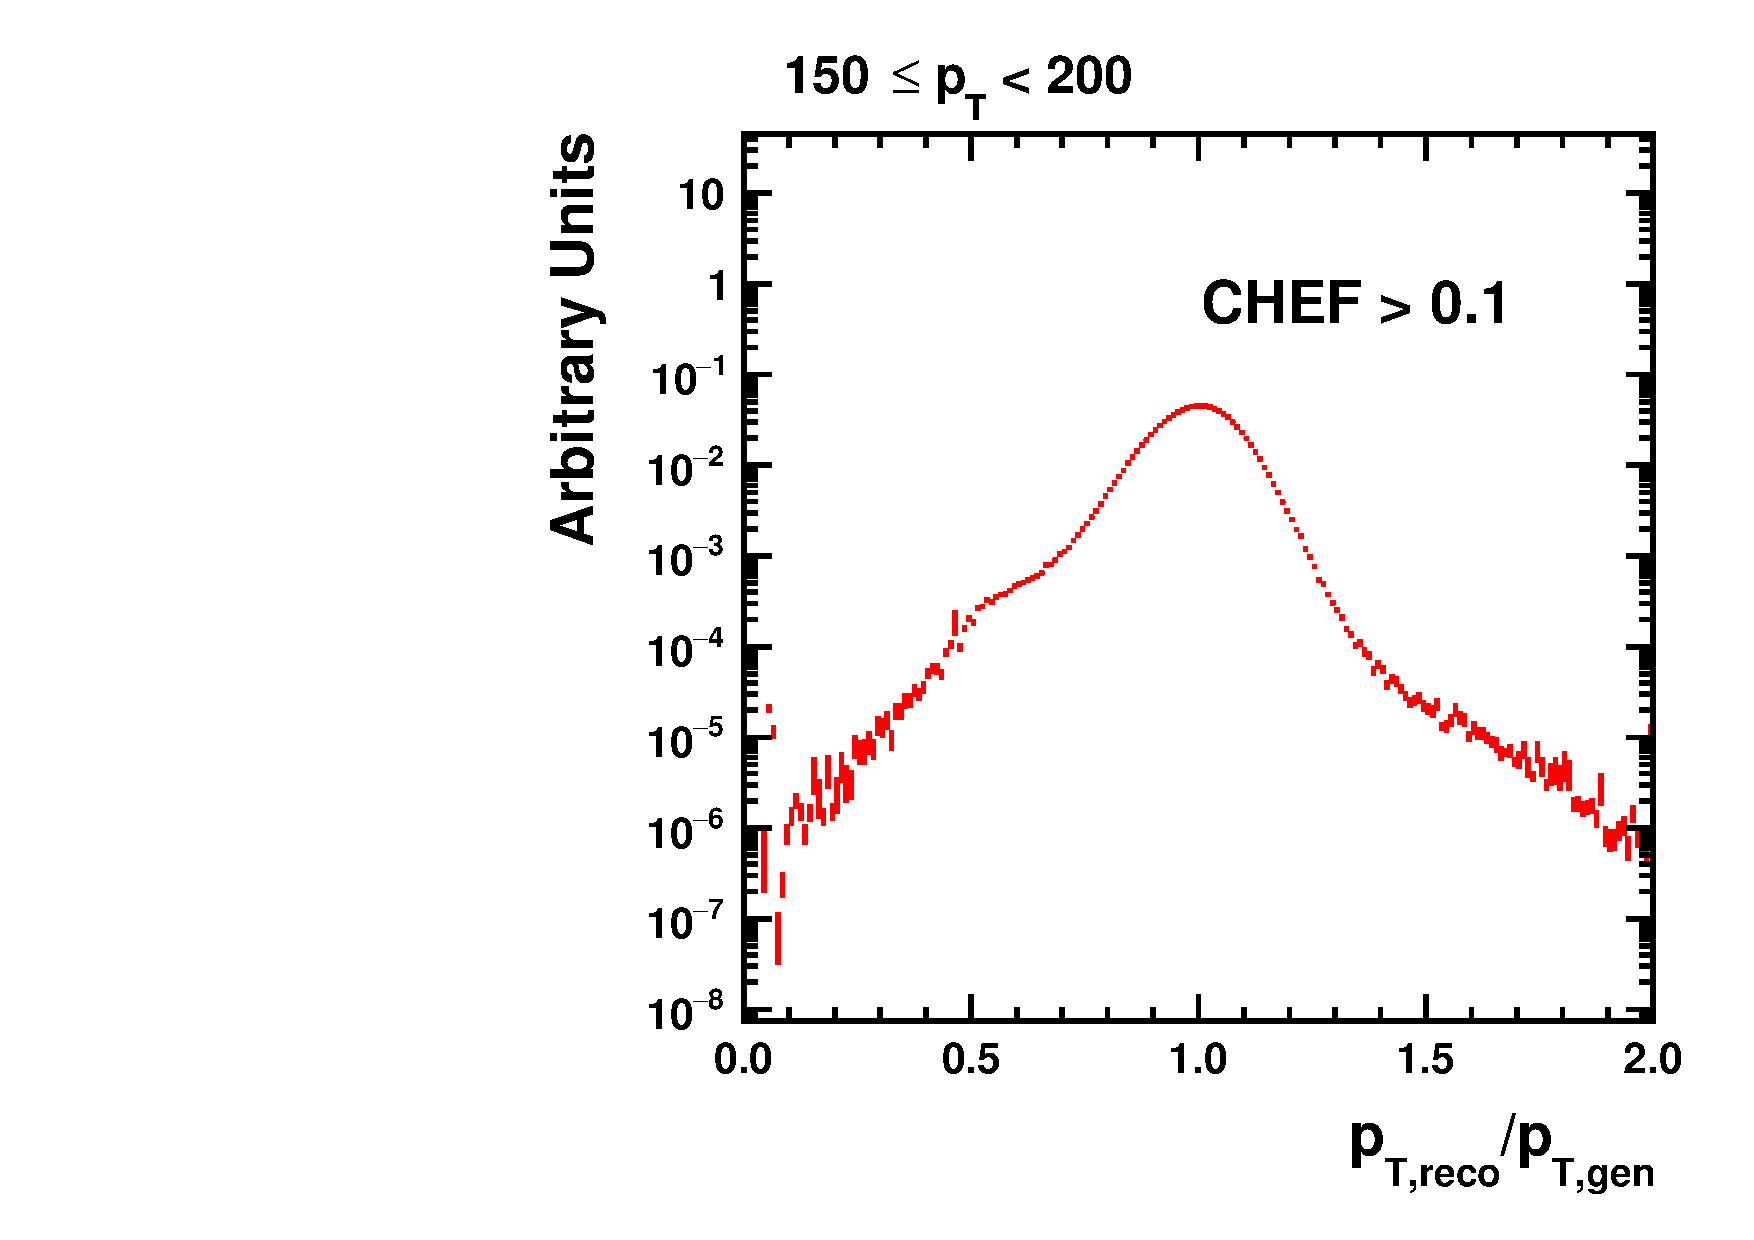
\includegraphics[width=0.25\textwidth]{diagnostics_NANO/res_b_NANO_6.pdf} \\
  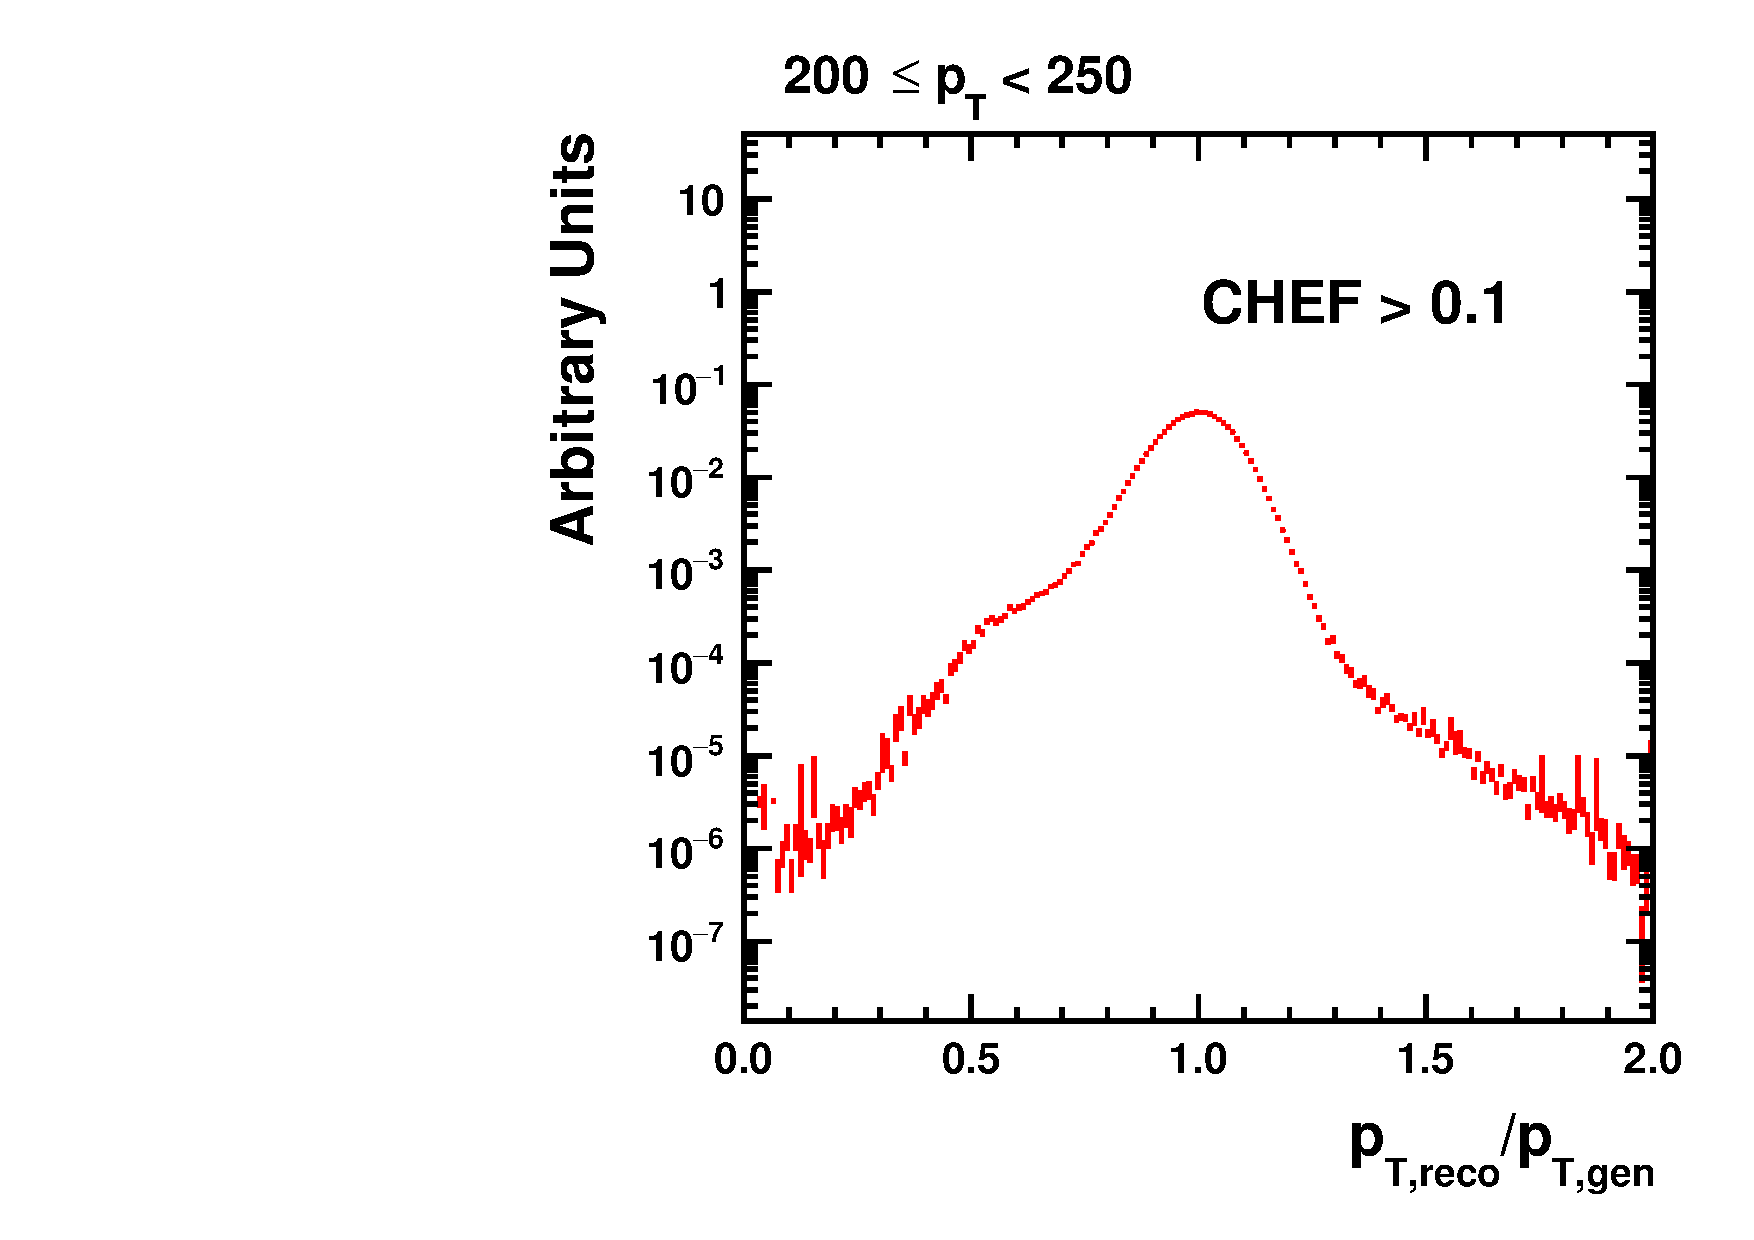
\includegraphics[width=0.25\textwidth]{diagnostics_NANO/res_b_NANO_7.pdf}
  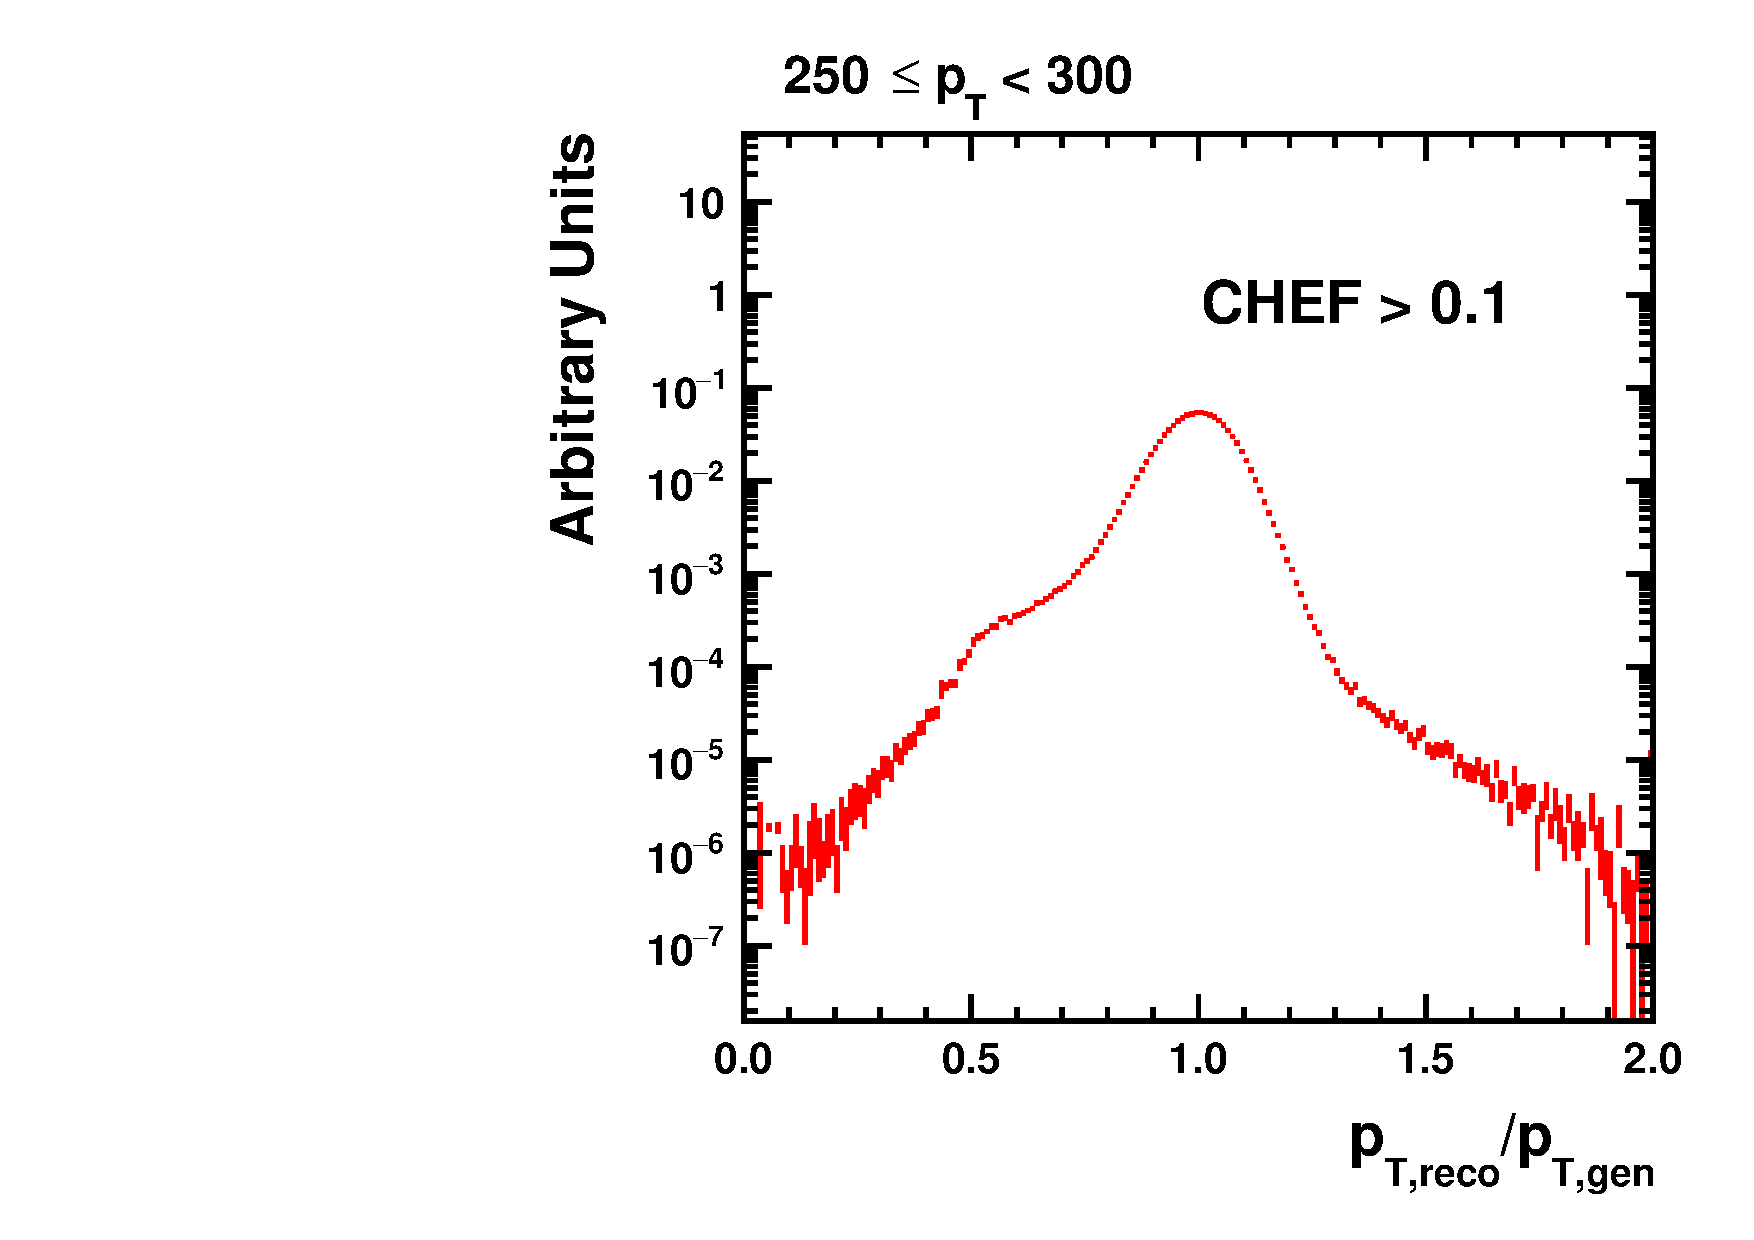
\includegraphics[width=0.25\textwidth]{diagnostics_NANO/res_b_NANO_8.pdf} 
  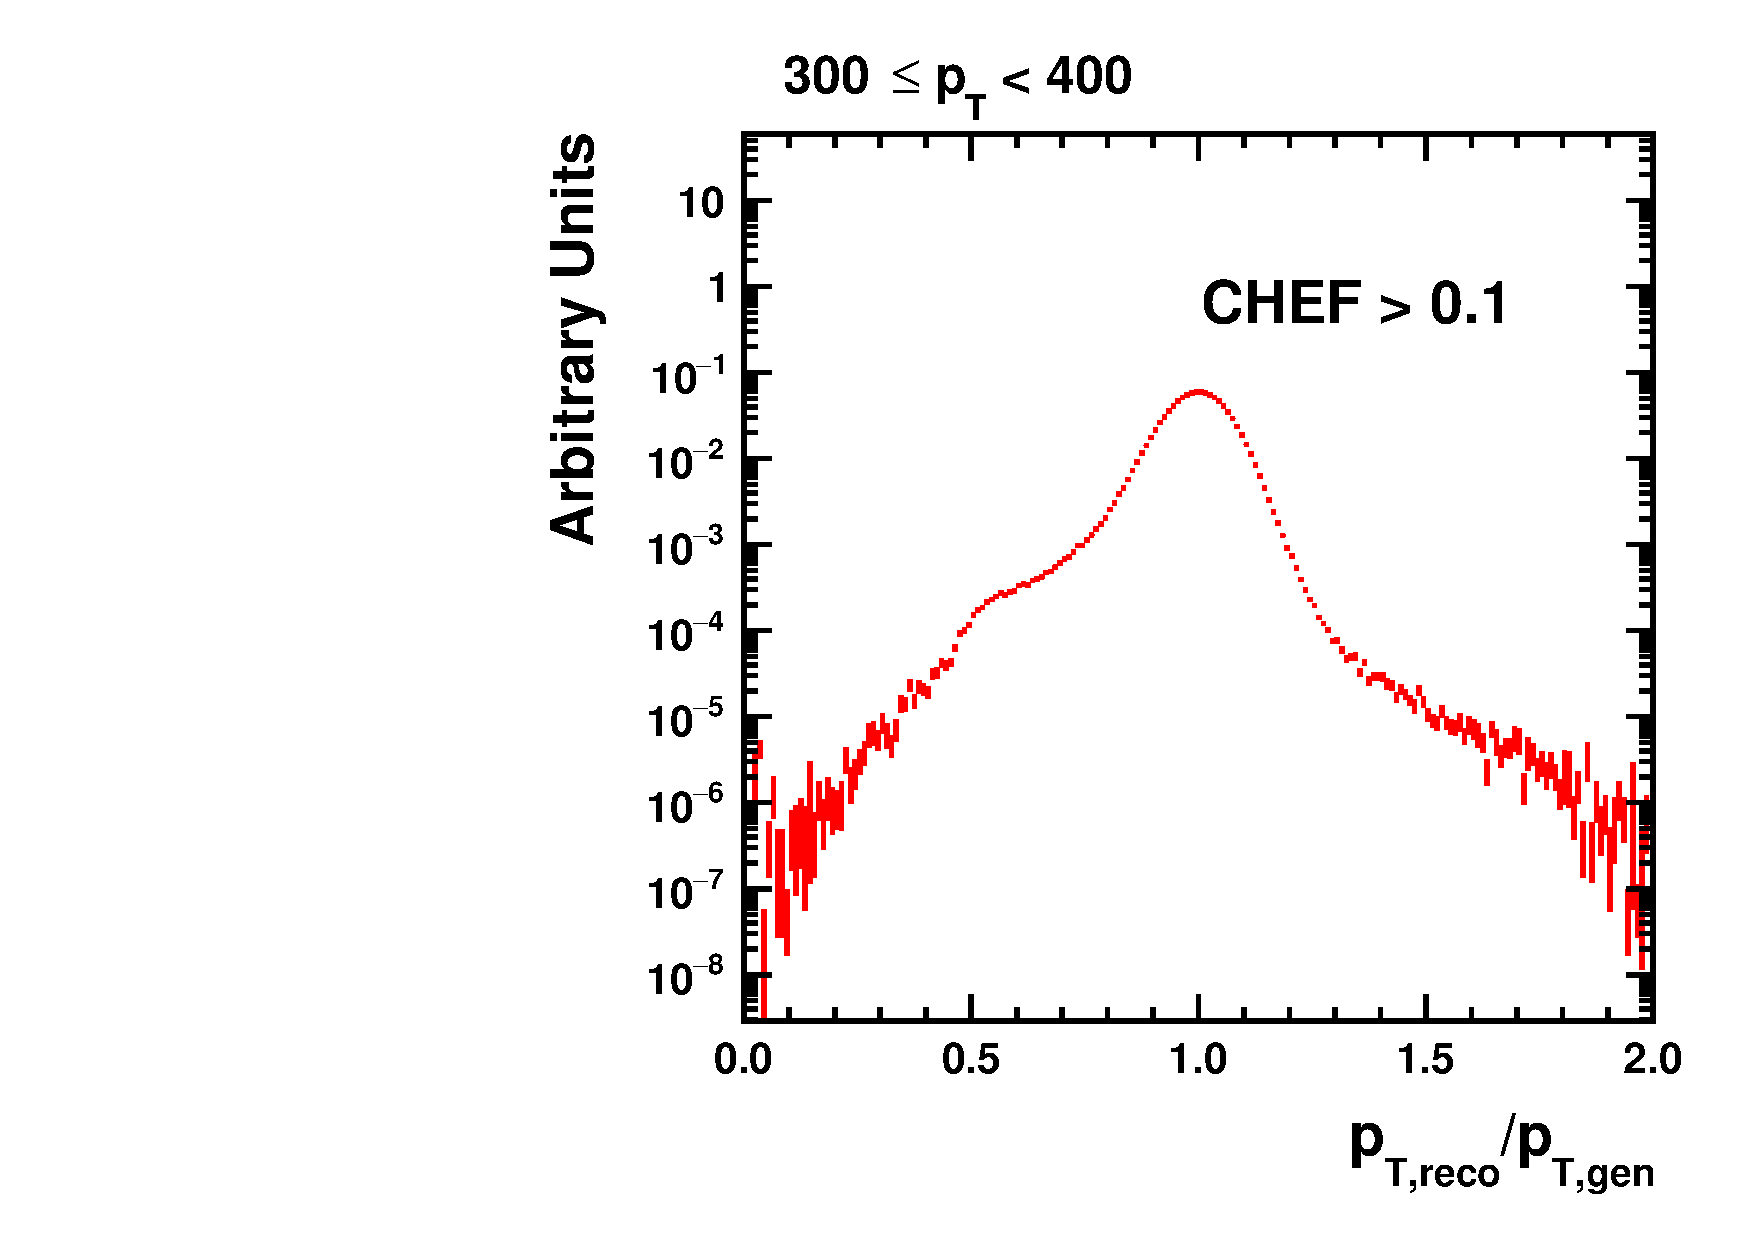
\includegraphics[width=0.25\textwidth]{diagnostics_NANO/res_b_NANO_9.pdf} \\
  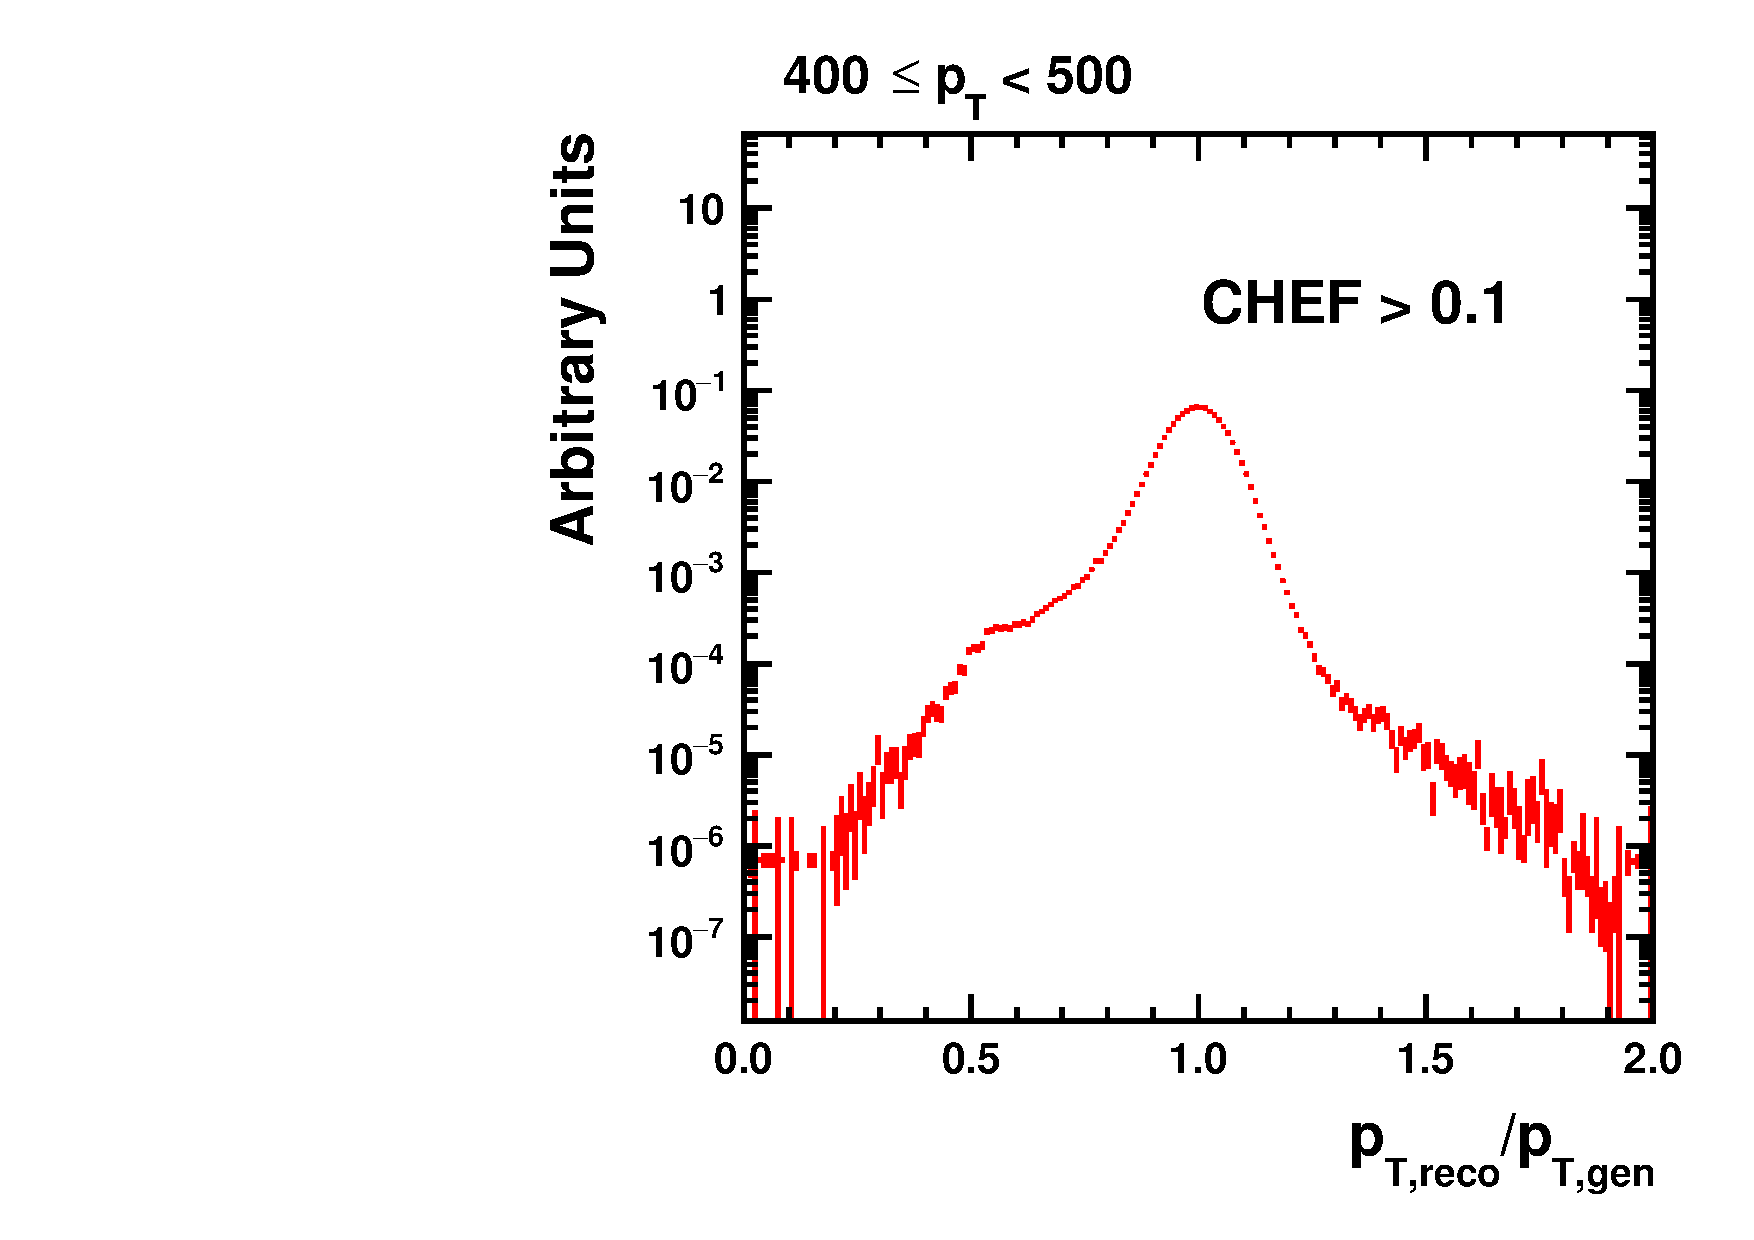
\includegraphics[width=0.25\textwidth]{diagnostics_NANO/res_b_NANO_10.pdf}
  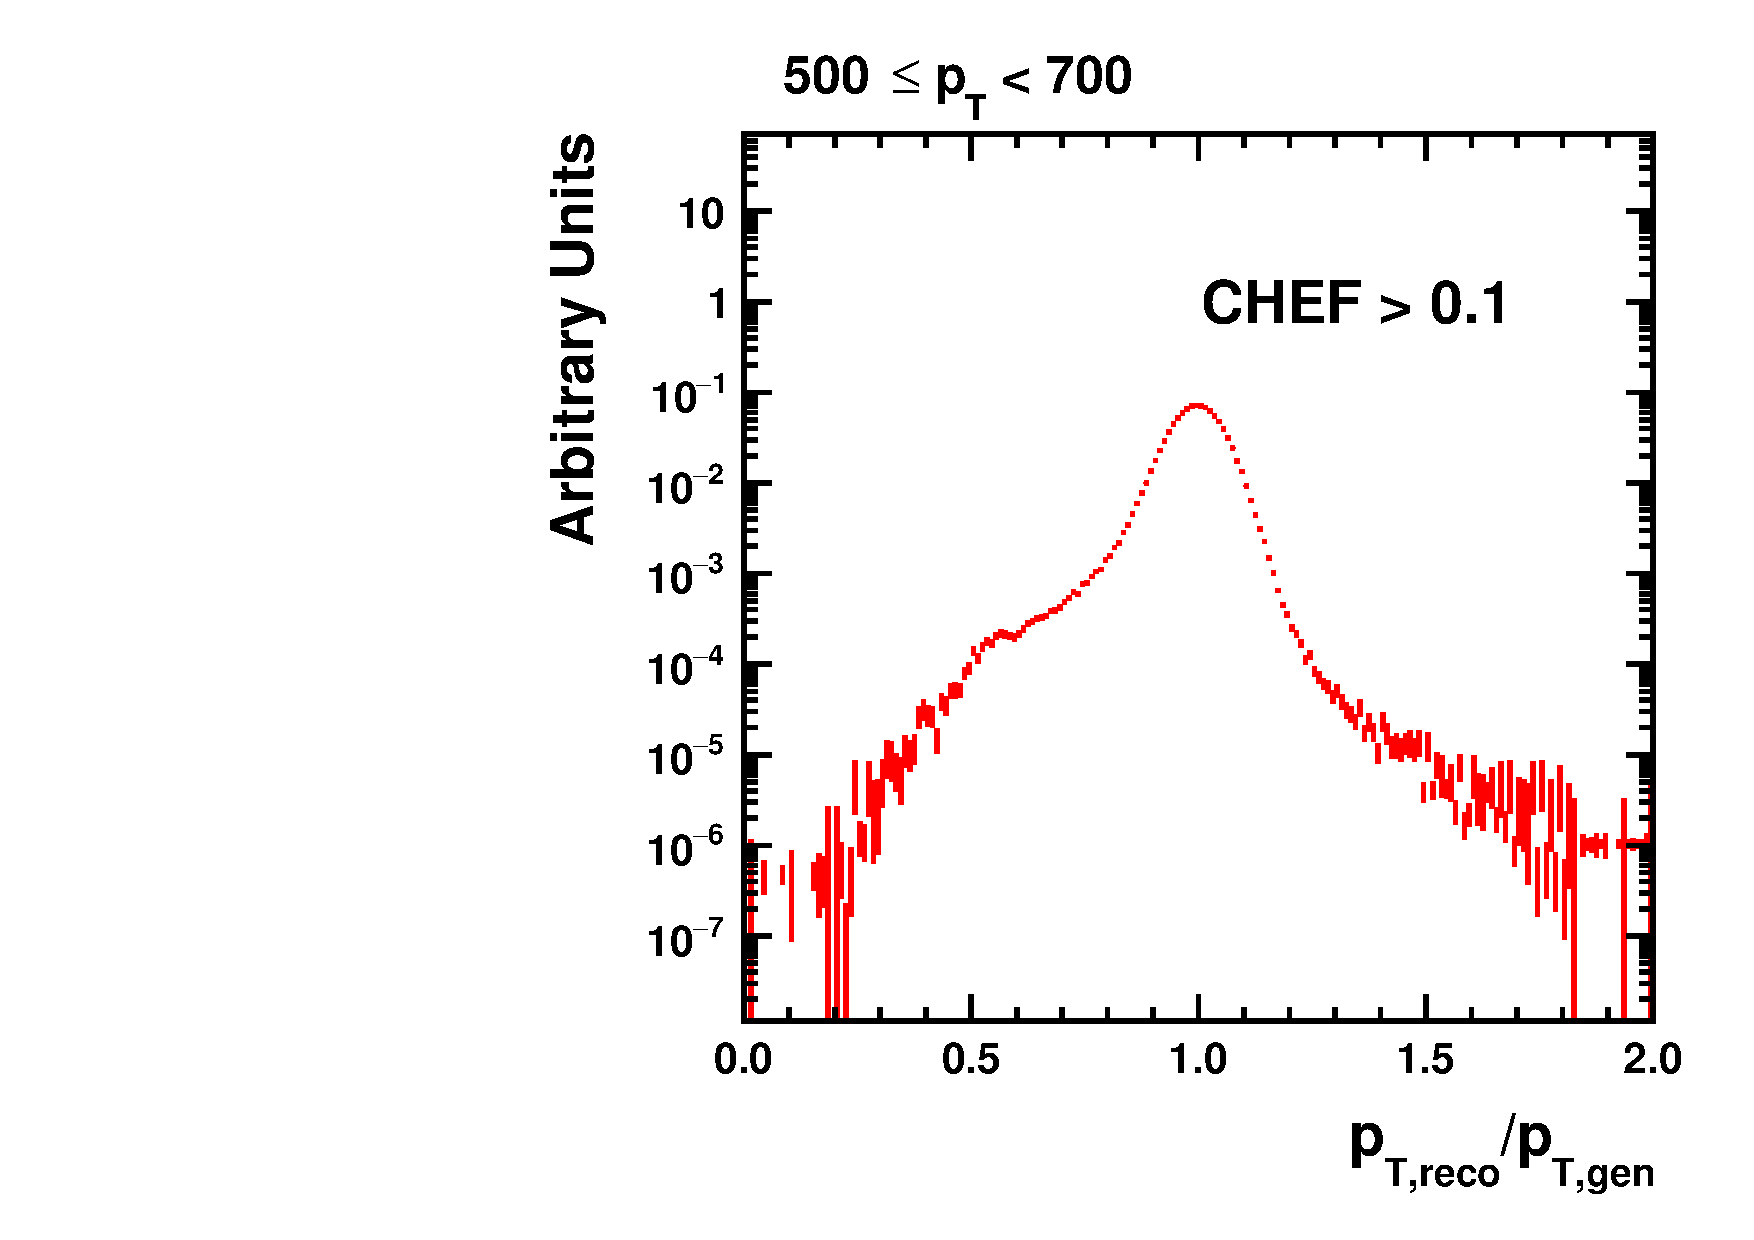
\includegraphics[width=0.25\textwidth]{diagnostics_NANO/res_b_NANO_11.pdf} 
  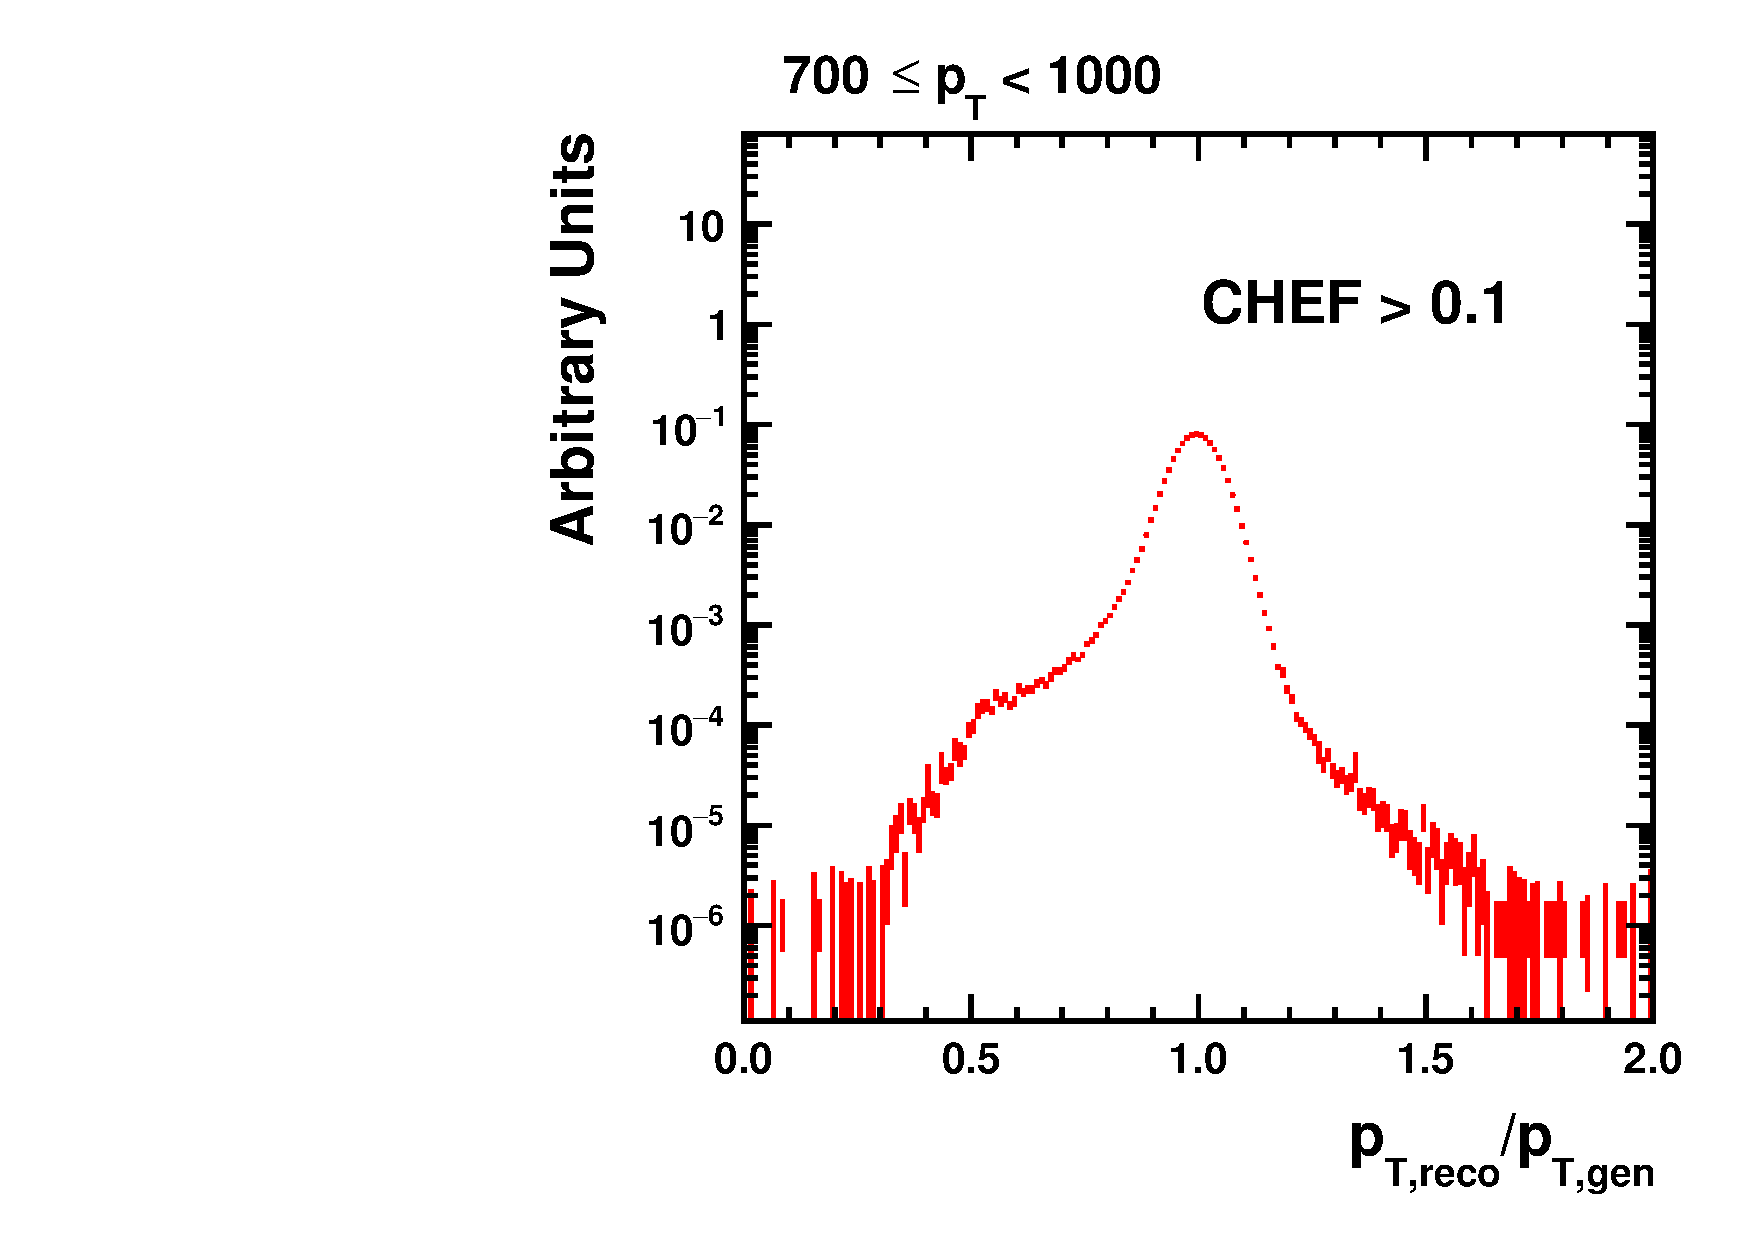
\includegraphics[width=0.25\textwidth]{diagnostics_NANO/res_b_NANO_12.pdf}     
  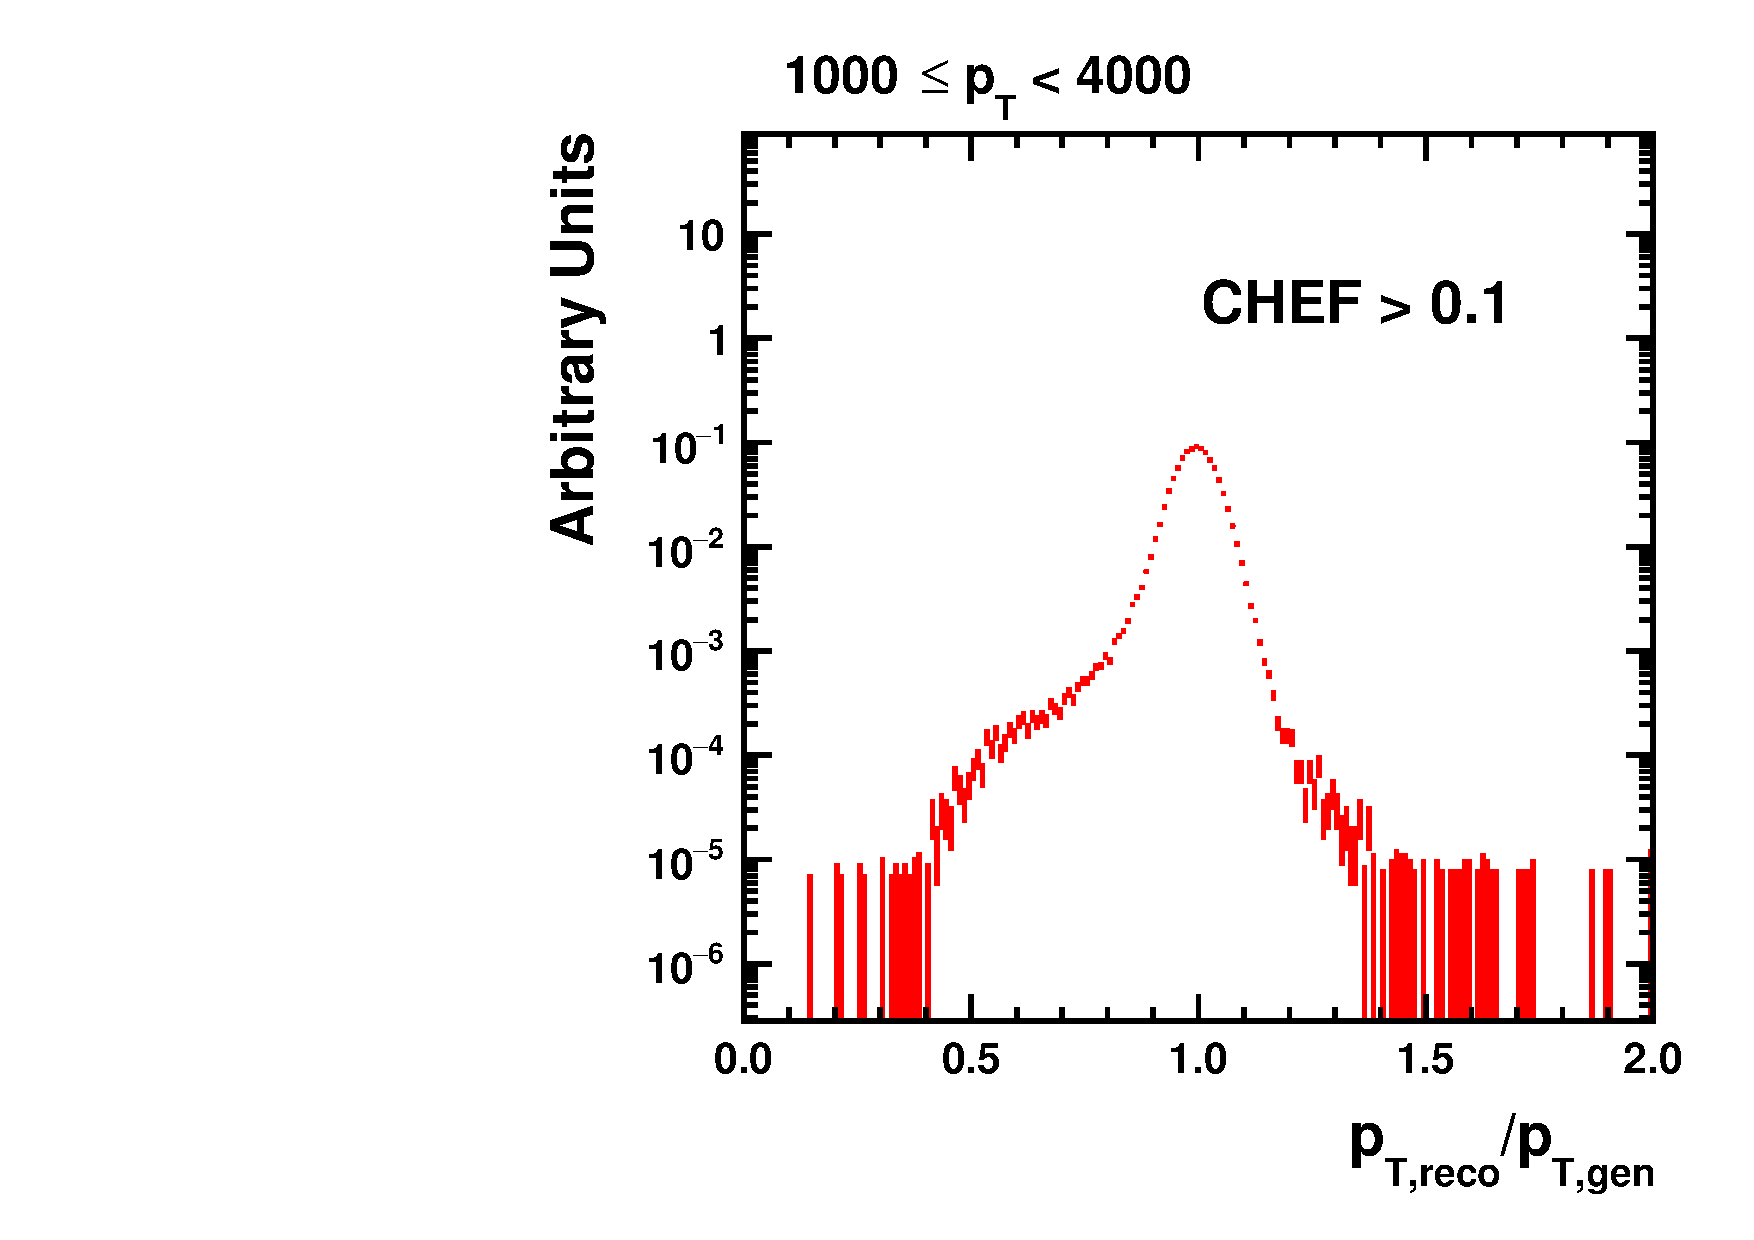
\includegraphics[width=0.25\textwidth]{diagnostics_NANO/res_b_NANO_13.pdf} \\ 
	\end{center}
	\caption[B Jet Response]{Comparison of the Data and MC in the 1Lep CR for each era: Run2016, Run2017BtoE, Run2017F, Run2018preHEM, Run2018PostHEM, and the combination of all eras in the High \dm{} region. Each era has a good agreement between Data and MC. 
	 }
	\label{fig:qcd-1lcr-datavsmc-hm-inclusive}
\end{figure}
